\documentclass[11pt]{article}
\usepackage[T1]{fontenc}
\usepackage[utf8]{inputenc}
\usepackage{lmodern}
\input{glyphtounicode}
\input{glyphtounicode-cmex}
\pdfgentounicode=1
\pdftrailerid{}
\usepackage[margin=1in]{geometry}
\usepackage{amsmath,amssymb,amsthm,mathtools,mathrsfs}
\usepackage{microtype,enumitem,booktabs,array,longtable,needspace}
\usepackage{tikz}
\usetikzlibrary{arrows.meta,positioning}
\usepackage{xcolor}
\usepackage{xurl}
\usepackage{hyperref}
\hypersetup{colorlinks=true,linkcolor=blue!45!black,citecolor=blue!45!black,
urlcolor=blue!45!black,pdftitle={Balanced counterexamples to Ryser's conjecture at prime orders},pdfauthor={OpenAI}}
\urlstyle{same}
\setlength{\emergencystretch}{2em}
\setlist{itemsep=3pt,topsep=5pt}
\newtheorem{theorem}{Theorem}[section]
\newtheorem{lemma}[theorem]{Lemma}
\newtheorem{proposition}[theorem]{Proposition}
\newtheorem{corollary}[theorem]{Corollary}
\theoremstyle{definition}
\newtheorem{definition}[theorem]{Definition}
\theoremstyle{remark}
\newtheorem{remark}[theorem]{Remark}
\newcommand{\F}{\mathbb F}
\newcommand{\E}{\mathbb E}
\newcommand{\Prb}{\mathbb P}
\DeclareMathOperator{\Var}{Var}
\DeclareMathOperator{\Cov}{Cov}
\title{Balanced counterexamples to Ryser's conjecture at prime orders}
\author{OpenAI}
\date{September 27, 2026}
\begin{document}
\maketitle
\begin{abstract}
For every sufficiently large prime $q$, we construct a finite intersecting
$(q+1)$-partite $(q+1)$-uniform hypergraph with covering number $q+1$
and exactly $q+1$ nonisolated vertices in each part. This disproves
Ryser's covering conjecture, even for intersecting hypergraphs with
equally sized parts.
\end{abstract}

\section{Introduction}

A vertex cover of a finite hypergraph $H$ is a set of vertices meeting
every edge. Its minimum possible size is the \emph{covering number}
$\tau(H)$. The \emph{matching number} $\nu(H)$ is the maximum number of
pairwise disjoint edges. For an integer $r\ge2$, an $r$-partite
$r$-uniform hypergraph has disjoint vertex parts $V_1,\ldots,V_r$, and
each edge contains exactly one vertex from each part. Here \emph{balance}
refers to equal sizes of the vertex parts. Ryser's covering conjecture
proposes that every such hypergraph satisfies
\begin{equation}\label{eq:ryser}
 \tau(H)\le (r-1)\nu(H).
\end{equation}
A hypergraph with at least one edge is \emph{intersecting} if every two
distinct edges meet. In this case $\nu(H)=1$, and the proposed bound is $r-1$.
A cover may use vertices from any of the parts, so making each individual
part large does not by itself obstruct a small cover.

For $r=2$, inequality~\eqref{eq:ryser} is K\H{o}nig's matching theorem
for bipartite graphs. Henderson's 1971 thesis contains an equivalent
formulation of the general conjecture~\cite{Henderson1971}; Best and
Wanless~\cite{BestWanless2018} discuss its attribution to Ryser and
separate it from his Latin-square transversal conjecture.
Aharoni proved the full tripartite case~\cite{Aharoni2001}.
In the intersecting case, Gy\'arf\'as proved the conjecture through rank
four and Tuza proved rank five; see
Kir\'aly and T\'othm\'er\'esz~\cite{KiralyTothmeresz2017} for the
historical account. For \emph{linear} intersecting hypergraphs, in which
every two distinct edges meet in exactly one vertex, Franceti\'c, Herke,
McKay, and Wanless established the conjecture through rank
nine~\cite{FranceticHerkeMcKayWanless2017}.
For each of $r=4,5$, Haxell and Scott proved a bound
$\tau(H)\le(r-\varepsilon_r)\nu(H)$ with a positive constant
$\varepsilon_r$~\cite{HaxellScott2012}. More recently, White proved
$\tau(H)\le6$ for four-partite four-uniform hypergraphs with
$\nu(H)=2$~\cite{White2026}.
These results concern the covering inequality itself. Lov\'asz proposed
the stronger assertion that, in every $r$-partite $r$-uniform hypergraph
with at least one edge, deleting $r-1$ vertices can reduce the matching number.
Clow, Haxell, and Mohar disproved that assertion at
$r=3$~\cite{ClowHaxellMohar2025}; Abiad, Garbe, Povill, and Spiegel
subsequently gave an infinite family at $r=3$ and examples at
$r=4$~\cite{AbiadGarbePovillSpiegel2025}. Those examples do not
contradict~\eqref{eq:ryser}.

Finite planes explain why the bound $r-1$ is natural. In the affine plane
$\F_q^2$, make one part for each of the $q+1$ directions, with one vertex
for each line of that direction. An affine point determines an edge
consisting of the labels of the lines through it. Two such edges meet at
the label of their joining line. Each parallel class is a cover of size
$q$, and fewer than $q$ lines cannot cover $q^2$ points. Thus this
hypergraph is intersecting and has covering number $q$. It is the usual
truncated-projective-plane example, expressed through affine duality.

Abu-Khazneh, Bar\'at, Pokrovskiy, and Szab\'o exploit the rigidity of
minimum covers in a truncated plane and add a new part and exceptional
edges. For every prime power $q\ge3$, their construction yields an
intersecting $(q+2)$-partite $(q+2)$-uniform hypergraph with covering
number $q+1$~\cite[Theorem~1.2, Lemma~1.3, Corollary~1.4]{AbuKhaznehBaratPokrovskiySzabo2019}.
Haxell and Scott use affine planes to construct intersecting $r$-partite
$r$-uniform hypergraphs with covering number at least $r-4$ for every
sufficiently large $r$, and at least $r-3$ when $r$ is
even~\cite[Theorem~6]{HaxellScott2017}.

Equal part sizes alone do not force a large covering number:
Franceti\'c, Herke, McKay, and Wanless constructed a linear intersecting
13-partite hypergraph with 13 nonisolated vertices in each part, and
reported that its covering number is nine by
computation~\cite[Section~3.1]{FranceticHerkeMcKayWanless2017}.
Here we modify the affine-plane example while keeping $q+1$ parts, one
for each direction. The modification raises both the covering number and
each part size to $q+1$.

\begin{theorem}\label{thm:main}
There exists $q_0$ such that, for every prime $q\ge q_0$, there is a
finite intersecting $(q+1)$-partite $(q+1)$-uniform hypergraph $H$ with
\[
 |V_1|=\cdots=|V_{q+1}|=q+1,
 \qquad \tau(H)=q+1.
\]
Every vertex belongs to an edge.
\end{theorem}

Since $\nu(H)=1$, this gives counterexamples to~\eqref{eq:ryser}.
The value $\tau(H)=r$, where $r=q+1$, is the largest possible for an
intersecting $r$-uniform hypergraph, since any edge is a cover. The
nonisolated vertices in each part also form a cover, so a hypergraph with
$\tau(H)=r$ must have at least $r$ such vertices in every part. Our
construction attains this minimum simultaneously in all parts.

The argument produces an example for each prime beyond one fixed
threshold; that threshold is not numerical.
The companion article~\cite[Theorem~1.1]{OpenAIExtension2026} treats a different
range of field orders: for every sufficiently large prime $s\equiv2
\pmod3$, it gives counterexamples of order $q=s^n$ for every sufficiently
large odd $n$, with the threshold for $n$ depending on $s$. Its theorem
does not assert balance. The proof here is independent of that
construction.

\subsection{Monochromatic tree covers}

An $r$-edge-coloring assigns one of $r$ colors to each edge of a graph.
A monochromatic tree cover is a family of monochromatic trees whose
vertex sets cover the graph; overlaps and singleton trees are allowed.
Gy\'arf\'as's tree-cover conjecture asks for at most $r-1$ such trees
in every $r$-edge-colored complete graph
\cite[Conjecture~1]{Milicevic2017}. Erd\H{o}s, Gy\'arf\'as, and Pyber
record the equivalence of this covering formulation with the
intersecting case of Ryser's conjecture
\cite[Section~3, after Theorem~2]{ErdosGyarfasPyber1991}. The standard
transfer gives the following consequence of Theorem~\ref{thm:main}.

\begin{corollary}\label{cor:tree-cover}
For every sufficiently large prime $q$, there is a finite complete
graph with a $(q+1)$-edge-coloring whose vertices require exactly
$q+1$ monochromatic trees to cover. The same minimum holds for
connected monochromatic subgraphs.
\end{corollary}
\begin{proof}
Put $r=q+1$ and take the hypergraph $H$ from Theorem~\ref{thm:main}.
Use its edges as the vertices of a complete graph. Color a pair
$ef$ by any index $i$ for which $e$ and $f$ have the same vertex in
part $V_i$; intersection guarantees such an index. Along a path of
color $i$, this vertex of $V_i$ is constant. Thus each connected
monochromatic subgraph corresponds to a hypergraph vertex lying in all
the hyperedges represented by its vertices; for a singleton choose any
vertex of the corresponding hyperedge.
A cover by $t$ such subgraphs would give a vertex cover of $H$ of
size at most $t$, so $t\ge\tau(H)=r$. Conversely, the $r$
monochromatic stars centered at any fixed graph vertex cover the
complete graph, allowing singleton stars for unused colors.
\end{proof}

\subsection{Balance, intersection, and the cover obstruction}

The affine-plane example starts with $q$ blocks in each parallel class.
We replace those line partitions by partitions with $q+1$ blocks, keeping
one vertex part for each direction. In a given direction, merge two
parallel lines into one block, and split two other parallel lines into
two blocks each. The count becomes
\[
 (q-4)+1+4=q+1.
\]
Each split line keeps just four designated points. Writing them in a
cyclic order as $u_0,u_1,u_2,u_3$, its blocks are the opposite pairs
$\{u_0,u_2\}$ and $\{u_1,u_3\}$. All points outside the chosen split
lines are retained as well. The choices ensure that designated points
lie on no other chosen split line, so these rules really give partitions
of one common set of retained points. The blocks label vertices and the
retained points label edges.

The splitting operation creates the first difficulty: two points on a
split line may now have different labels in that direction. We arrange
four merged pairs in four distinct other directions so that each
consecutive pair $u_{i-1},u_i$ lies in a common merged block. These are
exactly the pairs separated by the opposite-pair partition. Thus every
pair of retained points still shares a block somewhere, and the resulting
hypergraph remains intersecting. Figure~\ref{fig:cycle} shows the rule;
Section~\ref{sec:deterministic-construction} states its precise incidence
and compatibility requirements.

The harder difficulty is to rule out a cover using labels from several
parts. Temporarily remove all split lines and one constituent of each
merged pair. On the surviving \emph{core}, every remaining block is
represented by a single ordinary line. Hence a cover with at most $q$
labels gives a cover of the core by at most $q$ lines. We prove that
almost all those lines belong to one \emph{projective pencil}: they pass
through one affine point, or are all parallel if the common projective
point is at infinity.

Every relevant line also retains a positive proportion of its points.
This occupancy forces a hypothetical cover to select every nonsplit
member of its pencil. Only a small budget of labels remains for the
four-point sets on split lines through the pencil's center. Compatibility
handles the parallel case and pencils containing at most two split
lines. For larger pencils, a separate incidence count shows that the
remaining budget is insufficient. The deterministic result in
Section~\ref{sec:deterministic-construction} makes these requirements
explicit before we construct data satisfying them.

\subsection{Producing the geometric data}

The probabilistic argument has to preserve its estimates through several
choices. First sample two independent constituent lines in each
direction. They generate many candidate four-point tuples on different
split lines. An incompatibility graph records choices that cannot coexist.
There are two slots per direction, each carrying the candidates for one
split line. Choosing one candidate in every slot without an incompatible
pair is an \emph{independent transversal} of this graph.

Section~\ref{sec:candidates} bounds the sizes and degrees of this graph,
including the exceptional pairs that can have large common neighborhoods.
Section~\ref{sec:selection} then constructs a random independent
transversal while maintaining line occupancy. The procedure first makes
random choices and adds thinning to equalize one-step survival; it completes
the last slots using the local lemma. Partial random selection followed
by local-lemma completion also appears in the locally sparse transversal
argument of Loh and Sudakov~\cite[Section~4]{LohSudakov2007}.
Here we need an additional quantitative output: prescribing the choices
in $s$ slots, jointly with successful return, has probability at most
$(K_*/q)^s$ for a fixed constant $K_*$. This bound controls later
incidence counts without assuming that selected tuples are independent.

The core estimate in Section~\ref{sec:deletion} is designed for the law
of these selected lines. Under uniform deletion of a fixed number of
lines per direction, with probability tending to one every small core
cover also covers almost all of the whole plane. The key counting lemma bounds forbidden profile classes by
$\exp(-\Omega(q\log q))$. After the preliminary density and occupancy
restrictions are imposed, this saving pays for both the possible covers
and the $\exp(O(q))$ change of measure introduced by selection; the
resulting almost-cover conclusion holds with probability tending to one
under the changed law. Random line constructions and the counting of small covers through collinear subsets
have precedents in Erd\H{o}s and Lov\'asz~\cite[Section~4]{ErdosLovasz1975};
Kahn subsequently developed the random-line approach
further~\cite{Kahn1992}. The profile argument here supplies the
change-of-measure control needed for our selection law.
We then apply the prime-plane stability theorem of Sz\H{o}nyi and
Weiner~\cite{SzonyiWeiner2012}, also stated by H\'eger and
Nagy~\cite{HegerNagy2017}, to turn an almost-cover into a large pencil.
This is the step that requires $q$ to be prime.

Finally, Section~\ref{sec:pencils} combines the prescribed-choice bound
with the original independent constituent offsets. It counts repeated
generator directions and the additional incidences that a small local
cover would require. Section~\ref{sec:assembly} intersects the resulting
successful events and applies the deterministic construction.
Appendix~\ref{sec:elementary} supplies three elementary estimates in a
form independent of the construction; these are also the precise inputs
used by the companion article.

\paragraph{Conventions.}
All logarithms are natural. An event holds with high probability if its
probability tends to one along the orders under discussion. Constants
in $O(\cdot)$ may depend on parameters fixed before $q$ varies. Every
auxiliary constant is fixed independently of $q$; the final threshold
may depend on those constants.

\section{From modified line partitions to a hypergraph}
\label{sec:deterministic-construction}

The geometric data needed for the theorem have two jobs: preserve the
intersection of point-edges after lines are split, and rule out every
cover using at most $q$ block labels. We formulate both requirements here
and prove that they suffice. The later probabilistic sections will produce
the data; all arguments in this section are deterministic and work over
any finite field.

Let $q\geq4$ be a prime power, let $A=\mathbb F_q^2$, and let
$\mathcal G$ be the set of its $q+1$ directions.  For $g\in\mathcal G$,
write $\mathcal L_g$ for the $q$ affine lines of direction $g$, and put
$\mathcal L=\bigcup_g\mathcal L_g$.  The affine line of direction $g$
through $p\in A$ is denoted by $p+g$.  We also use the projective completion
$\operatorname{PG}(2,q)$.  Thus a common projective point of affine lines
means either an ordinary point of concurrence or the point at infinity of
a parallel class.

\subsection{Merged pairs and four-point split lines}

For every direction $g$, choose two distinct lines
$M_g^0,M_g^1\in\mathcal L_g$.  Call their union the merged pair in
direction $g$, and call either of its lines a constituent.  Write
\[
 \mathcal M=\{M_g^s:g\in\mathcal G,\ s\in\{0,1\}\}.
\]
If $S\in\mathcal L_g\setminus\mathcal M$, define a simple graph on the
points of $S$: two distinct points are adjacent if they are the two
intersections of $S$ with $M_d^0,M_d^1$ for some $d\ne g$.  Several
directions may give the same adjacency; its multiplicity is irrelevant.

A tuple in direction $g$ consists of four distinct directions
$d_0,d_1,d_2,d_3\in\mathcal G\setminus\{g\}$ and four bits
$\sigma_0,\sigma_1,\sigma_2,\sigma_3\in\{0,1\}$.  Indices on the tuple
are read modulo $4$.  Define
\begin{equation}
 u_i=M_{d_i}^{\sigma_i}\cap M_{d_{i+1}}^{1-\sigma_{i+1}}.
 \label{eq:det-tuple-points}
\end{equation}
The intersections exist uniquely because consecutive generator directions
are different.  Call the tuple valid if the following conditions hold:
\begin{enumerate}
 \item Its four points are distinct and lie on one line
 $S\in\mathcal L_g\setminus\mathcal M$.
 \item Neither $\{u_0,u_2\}$ nor $\{u_1,u_3\}$ is an adjacency on $S$.
 \item Every point of $S\setminus\{u_0,u_1,u_2,u_3\}$ is adjacent to at
 most one of $u_0,u_1,u_2,u_3$.
\end{enumerate}
We call $S$ its split line and write $F_S=\{u_0,u_1,u_2,u_3\}$.  Each
consecutive pair $\{u_{i-1},u_i\}$ is adjacent: the two points lie on the
two different constituents of direction $d_i$.  Consequently the two
opposite pairs partition $F_S$, and every pair crossing that partition
shares a merged pair.

Figure~\ref{fig:cycle} records the partition and the shared merged
blocks. The conditions on opposite pairs and external points will also
control covers centered at a point of $S$.

We need two split lines in every direction. Index these requirements by
slots $(g,s)$, where $g\in\mathcal G$ and
$s\in\{1,2\}$, and choose a valid tuple in each slot. Write $S_g^s$
for its split line.
The choices are \emph{compatible} if the following conditions hold for
any two different slots:
\begin{enumerate}
 \item Neither chosen split line contains a designated point of the other
 tuple.
 \item The two sets of generator directions have intersection of size at
 most one.
 \item If the slots have the same target direction, no merged pair
 contains at least two designated points of one tuple and at least one
 designated point of the other.
\end{enumerate}
The first condition makes all chosen split lines distinct and makes their
designated point sets pairwise disjoint.  In particular, there are exactly
two split lines in each direction, both different from its two
constituents.  The second condition will be relevant to constructing such
data; the deterministic implication below uses the first and third
conditions.

\begin{figure}[htbp]
\centering
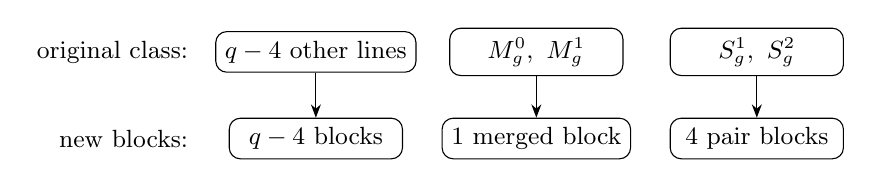
\begin{tikzpicture}[font=\small]
\node[anchor=east] at (-.2,1.1) {original class:};
\node[draw,rounded corners,minimum width=2.2cm] (ordinary) at (1.3,1.1)
 {$q-4$ other lines};
\node[draw,rounded corners,minimum width=2.2cm] (merged) at (4.1,1.1)
 {$M_g^0,\ M_g^1$};
\node[draw,rounded corners,minimum width=2.2cm] (split) at (6.9,1.1)
 {$S_g^1,\ S_g^2$};
\node[anchor=east] at (-.2,0) {new blocks:};
\node[draw,rounded corners,minimum width=2.2cm] (ordinary2) at (1.3,0)
 {$q-4$ blocks};
\node[draw,rounded corners,minimum width=2.2cm] (merged2) at (4.1,0)
 {$1$ merged block};
\node[draw,rounded corners,minimum width=2.2cm] (split2) at (6.9,0)
 {$4$ pair blocks};
\draw[-{Stealth}] (ordinary)--(ordinary2);
\draw[-{Stealth}] (merged)--(merged2);
\draw[-{Stealth}] (split)--(split2);
\end{tikzpicture}

\medskip
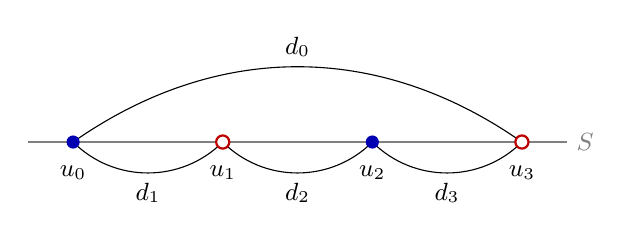
\begin{tikzpicture}[scale=.95,font=\small]
\draw[gray] (-.6,0)--(6.6,0) node[right] {$S$};
\foreach \i/\x in {0/0,1/2,2/4,3/6}{
 \coordinate (u\i) at (\x,0);
 \node[below=5pt] at (u\i) {$u_\i$};}
\draw (u0) to[bend right=45] node[below] {$d_1$} (u1);
\draw (u1) to[bend right=45] node[below] {$d_2$} (u2);
\draw (u2) to[bend right=45] node[below] {$d_3$} (u3);
\draw (u3) to[bend right=35] node[above] {$d_0$} (u0);
\foreach \i in {0,2}{\fill[blue!70!black] (u\i) circle (2.5pt);}
\foreach \i in {1,3}{\draw[red!75!black,thick,fill=white] (u\i) circle (2.5pt);}
\end{tikzpicture}
\caption{The merge and split operation gives $q+1$ blocks per direction.
Below, the four points on one split line form two opposite-pair blocks,
shown by filled and open points. An arc labelled $d_i$ means that its
endpoints lie on different constituents of the merged pair in direction
$d_i$, and hence share its block label. The arcs record this relation;
they are not affine lines. The diagram is schematic.}
\label{fig:cycle}
\end{figure}


Let $\mathcal S$ be the set of chosen split lines, and define
\begin{equation}
 \begin{split}
 D&=\mathcal S\cup\{M_g^1:g\in\mathcal G\},\\
 R_0&=A\setminus\bigcup_{\ell\in D}\ell,
 \qquad R=A\setminus\bigcup_{S\in\mathcal S}S,\\
 X&=R\cup\bigcup_{S\in\mathcal S}F_S.
 \end{split}
 \label{eq:det-core}
\end{equation}
There are exactly three lines of $D$ in each direction.  Compatibility
gives
\begin{equation}
 S\cap X=F_S\qquad(S\in\mathcal S).
 \label{eq:det-split-intersection}
\end{equation}
Indeed, $R$ contains no point of $S$, and no other designated point set
meets $S$.

The inclusion $R_0\subseteq R$ gives two retained sets with different purposes. On $R_0$, one
constituent of each merged block has disappeared, so a block cover becomes
an ordinary line cover. The larger set $R$ supplies points on the removed
constituents when we later force a cover to choose their merged blocks.
The four-point sets supply the final obstruction.

The following three properties express exactly what these sets must do.
Fix $0<\rho<1$ and an integer $B\geq0$.
\begin{description}
 \item[Occupancy.] At most $B$ constituent lines pass through any affine
 point.  Every $\ell\in\mathcal L\setminus D$ satisfies
 $|\ell\cap R_0|\geq\rho q$, and every $M_g^1$ satisfies
 $|M_g^1\cap R|\geq\rho q$.
 \item[Concentration of core covers.] If
 $C\subseteq\mathcal L\setminus D$, $|C|\leq q$, and the lines of $C$
 cover $R_0$, then at least $(1-\rho/4)q$ lines of $C$ pass through a
 common projective point.
 \item[The local condition.] For $p\in A$, define
 \[
  \mathcal S(p)=\{S\in\mathcal S:p\in S\},\qquad
  b(p)=|\mathcal S(p)|,\qquad F(p)=\bigcup_{S\in\mathcal S(p)}F_S,
 \]
 and
 \begin{equation}
 Z(p)=F(p)\cap
 \bigcup_{\substack{d\in\mathcal G,\ s\in\{0,1\}\\p\in M_d^s}}
 M_d^{1-s}.
 \label{eq:det-partner-set}
 \end{equation}
 Whenever $b(p)\geq3$, the set $F(p)$ cannot be covered by $Z(p)$ and
 at most $b(p)-1$ additional sets of the following types: sets of at most
 two points; affine lines outside $\mathcal S(p)\cup\mathcal M$; and
 merged pairs $M_d^0\cup M_d^1$, with no merged pair used more than once.
\end{description}
All these are properties of a specified finite configuration.  In
particular, none asserts that such a configuration exists.

\begin{proposition}[Deterministic reduction]
\label{prop:deterministic-reduction}
Let $q\geq4$ be a prime power.  Suppose a compatible collection of valid
tuples in $\mathbb F_q^2$ satisfies occupancy, concentration of core
covers, and the local condition with parameters $0<\rho<1$ and
$B\geq0$.  If
\begin{equation}
 \rho q>2(1+B),
 \label{eq:det-size-condition}
\end{equation}
then there is an intersecting $(q+1)$-partite $(q+1)$-uniform hypergraph
with exactly $q+1$ nonisolated vertices in each part and cover number
$q+1$.  Its edges are in bijection with the set $X$ in
\eqref{eq:det-core}.
\end{proposition}

\subsection{Partitions and intersecting edges}

We prove Proposition~\ref{prop:deterministic-reduction} in three stages:
construct the balanced partitions, reduce a small cover to one pencil,
and test the designated points against its remaining budget.

For each $g\in\mathcal G$, partition $X$ into these blocks:
\begin{itemize}
 \item $\ell\cap X$ for every regular line $\ell\in\mathcal L_g$,
 where ``regular'' excludes the two split lines and the two constituents
 in that direction;
 \item $(M_g^0\cup M_g^1)\cap X$;
 \item $\{u_0,u_2\}$ and $\{u_1,u_3\}$ for each of its two split lines,
 using that line's tuple ordering.
\end{itemize}
Distinct lines of $\mathcal L_g$ are disjoint and partition $A$, so
\eqref{eq:det-split-intersection} proves that these blocks partition $X$.
There are $(q-4)+1+4=q+1$ of them.  The split blocks have two points.
Every regular block is nonempty by the lower bound on $|\ell\cap R_0|$,
and the merged block is nonempty by the same lower bound for $M_g^0$.

Let $V_g$ consist of distinct labels for these blocks; choose disjoint
label sets for different directions.  A point $x\in X$ defines an edge
$e_x$ containing, for each $g$, the unique label of the block containing
$x$.  Thus every edge contains exactly one vertex from each of the $q+1$
parts.  Every label occurs in an edge because its block is nonempty.

For different $x,y\in X$, let $\ell$ be their joining line and let $g$
be its direction.  If $\ell$ is not a split line, then $x,y$ are in the
same regular or merged block of $V_g$.  If $\ell$ is a split line, both
points are designated by \eqref{eq:det-split-intersection}.  They either
belong to the same opposite-pair block or form consecutive positions in
its four-cycle.  In the latter case they share the merged block of the
corresponding generator direction.  Hence $e_x\cap e_y\ne\varnothing$.

Repeated edges would not affect the cover argument, but they do not
occur here.  If $e_x=e_y$ for different $x,y$, then in every direction
$h$ different from the direction of their joining line they lie on
different $h$-lines.  Their only possible common block in $V_h$ is
therefore the merged block.  The point $x$ would lie on a constituent in
each of these $q$ directions, contradicting $B<q$, which follows from
\eqref{eq:det-size-condition}.  Thus $x\mapsto e_x$ is injective.

Selecting labels covers all edges if and only if the corresponding
blocks cover $X$.  We will show that at least $q+1$ blocks are needed.
The reverse bound follows because all labels in any one part cover every
edge.

\subsection{Forcing the nonsplit members of a pencil}

We have obtained an intersecting hypergraph with the required part sizes
and no isolated vertices. Its covering number is the minimum number of
blocks covering $X$. We now use $R_0$ to locate any hypothetical small
cover, then use occupancy on $R_0$ and $R$ to force its nonsplit blocks.

Suppose that a collection $\mathcal B$ of at most $q$ labels covers $X$.
A split block misses $R_0$.  On $R_0$, a merged block is exactly
$M_g^0\cap R_0$, because $M_g^1\in D$.  Associate to each selected
regular block its line and to each selected merged block the line
$M_g^0$.  These representative lines are distinct, belong to
$\mathcal L\setminus D$, and cover $R_0$.  Concentration of core covers
provides a projective point $P$ lying on at least $(1-\rho/4)q$ selected
representatives.  Write $t$ for the number of selected labels that do not
have a representative through $P$, including all selected split labels.
Then
\begin{equation}
 t\leq\rho q/4.
 \label{eq:det-outside-pencil}
\end{equation}
We treat separately a parallel pencil and a pencil through an affine
point.

\paragraph{A point at infinity.}
Suppose $P$ is the point at infinity of direction $g$.  Every one of the
$q-3$ lines of $\mathcal L_g\setminus D$ must be a selected
representative.  Otherwise an omitted such line has at least $\rho q$
points in $R_0$, none covered by the parallel representatives through
$P$, while all remaining representatives cover at most $t$ of them.
Split blocks cover none of $R_0$, and $t<\rho q$.

The corresponding $q-3$ selected blocks cover none of the eight
designated points on the two split lines of direction $g$.  An additional
regular block covers at most one point on each of those lines, and a
split block has size two.  A merged pair of direction $g$ misses both
split lines.  A merged pair of any other direction has at most two
designated points on each split line; if it had at least three altogether,
it would have at least two on one and at least one on the other, contrary
to the third compatibility condition.  Thus every additional block
covers at most two of these eight points.  At most three labels remain
in the cover budget, so a cover is impossible.

\paragraph{An affine point.}
Now let $P=p\in A$.  We first show that for each direction $g$ such that
$p+g$ is not a split line, the selected labels must include its regular
block or, when $p+g$ is a constituent, its merged block.

If $\ell=p+g\notin D$ and its block is omitted, selected
representatives through $p$ cover at most the point $p$ on $\ell$.  All other
representatives cover at most another $t$ points there.  This contradicts
\[
 |\ell\cap R_0|\geq\rho q>1+\rho q/4\geq1+t.
\]
The strict inequality follows from \eqref{eq:det-size-condition}.

The only remaining nonsplit case is $\ell=p+g=M_g^1$.  Suppose its
merged block is omitted.  A selected regular block represented through
$p$ meets $\ell$ only possibly at $p$.  A selected merged block represented
through $p$ consists of a constituent $M_d^0$ through $p$ and its partner
$M_d^1$.  The former meets $\ell$ at $p$, and the latter contributes at
most one additional point.  None of these lines equals $\ell$, because
its own merged block was omitted.  There are at most $B$ such partners,
by the constituent multiplicity bound at $p$.  Hence all selected blocks
represented through $p$ cover at most $1+B$ points on $\ell$.  Every
other selected block covers at most two points on $\ell$: regular lines
meet it in at most one, merged pairs in at most two, and split blocks
have size two.  Occupancy on $R$ now gives the contradiction
\[
 \rho q\leq|\ell\cap R|
 \leq1+B+2t
 \leq1+B+\rho q/2
 <\rho q.
\]
This proves the claimed necessity of the block in every nonsplit
direction.

Put $b=b(p)$.  The split lines through $p$ have distinct directions,
because distinct parallel lines do not meet.  The claim therefore
requires $q+1-b$ distinct labels, leaving room for at most $b-1$ more.
It remains to check the designated points on those split lines.

\subsection{The remaining designated points}

For an affine center $p$, the nonsplit directions have forced $q+1-b$
labels, where $b=b(p)$. The possible cover therefore has at most $b-1$
labels left. The following cases show that the designated points on its
$b$ split lines cannot be covered within that budget.

If $b=0$, the required $q+1$ labels already exceed the budget.  If $b=1$,
write $S$ for the unique split line through $p$.  Exactly $q$ labels are
required, so no additional label is available.  On $F_S$ their blocks
can cover only $p$ itself, when $p\in F_S$, and points adjacent to $p$
on $S$: regular lines through $p$ supply only $p$, and a merged pair
through $p$ supplies only its partner intersection.  If $p=u_i$ is
designated, its opposite point $u_{i+2}$ is not adjacent to it and is
missed.  If $p\notin F_S$, validity allows at most one designated point
adjacent to $p$.  In either case $F_S$ is not covered.

Suppose now that $b\geq2$.  Compatibility implies that $p$ is not
designated on any split line through it: otherwise that point would lie
on a second chosen split line.  The designated sets on these lines are
pairwise disjoint, so $|F(p)|=4b$.  A required regular block through $p$
meets any such split line only at $p$ and therefore misses its designated
points.  A required merged block has one constituent through $p$ and
can cover designated points only with its partner.  Thus the required
blocks cover a subset of $Z(p)$.

For each $S\in\mathcal S(p)$, every point in $Z(p)\cap F_S$ is adjacent
to the external point $p$ in the graph on $S$.  Validity gives
$|Z(p)\cap F_S|\leq1$, and consequently
\begin{equation}
 |Z(p)|\leq b.
 \label{eq:det-partner-count}
\end{equation}
If $b=2$, at most one additional block is available.  A regular line
meets the two split lines in at most two points, a merged pair in at most
four, and a split block has two points.  Hence this extra block together
with $Z(p)$ covers at most $4+2<8=|F(p)|$ points.

Finally, let $b\geq3$.  Each of the at most $b-1$ additional labels is
represented on $F(p)$ by one of the sets allowed in the local condition:
a split block has two points, a regular line is outside
$\mathcal S(p)\cup\mathcal M$, and a merged block is contained in its
merged pair.  No merged pair is repeated because it has only one label.
The local condition therefore rules out covering $F(p)$.  This is the
last possible case, completing the proof of
Proposition~\ref{prop:deterministic-reduction}.

\begin{remark}
For the multiplicity bound $B=\lceil\log q\rceil$ used in the
probabilistic construction, it is enough to require explicitly
$q\geq4$ and $\rho q>2(1+\lceil\log q\rceil)$.  Every fixed
$\rho>0$ satisfies this inequality for all sufficiently large $q$.
Primality is not used in the deterministic reduction; any restriction
to prime orders must come from establishing the finite configuration
properties.
\end{remark}

\section{Deletion lines and concentration of core covers}
\label{sec:deletion}

The deterministic construction asks for rigidity of line covers of the
core $R_0$. We establish that rigidity in two steps. First, after a fixed
number of lines in each direction are deleted, with probability tending
to one every cover of the surviving set by at most $q$ other lines also
covers almost all of the plane. Second, over a prime field, the Sz\H{o}nyi--Weiner stability
theorem puts almost all lines of such an almost-cover in one pencil.

The deletion law matters. Our eventual split lines come from a constrained
selection, so their law is not uniform. We prove the first step for any
law whose probability at each deletion set is at most $\exp(Kq)$ times
its uniform probability, with $K$ fixed. A qualitative estimate for
uniform deletion would not suffice under this change of measure.

Throughout this section, $q$ tends to infinity through prime powers and
$A=\mathbb F_q^2$.  Let $\mathcal L$ be its $q(q+1)$ affine lines.  Primality
will be required only for the final application of projective stability.
Fix an integer $k\ge1$.  For $q\ge k$, let $\mathsf U_{q,k}$ be the uniform
law on sets $D\subseteq\mathcal L$ containing exactly $k$ lines in each
direction.  Define
\[
 R_D=A\setminus\bigcup_{\ell\in D}\ell,
 \qquad i_D(x)=|\{\ell\in D:x\in\ell\}|.
\]
For probability measures on a countable set, total variation distance is
one half of the sum of the absolute coordinate differences.

\begin{theorem}[Robust deletion estimates]\label{thm:deletion}
Fix $k\ge1$ and $K\ge0$.  For each $q$, let $\mathsf Q_q$ be a probability
law on the same sets as $\mathsf U_{q,k}$ such that
\[
 \mathsf Q_q(D)\le e^{Kq}\mathsf U_{q,k}(D)
 \quad\text{for every }D.
\]
Then the following assertions hold as $q\to\infty$.
\begin{enumerate}[label=\textup{(\roman*)}]
\item The empirical probability measure
$q^{-2}\sum_{x\in A}\delta_{i_D(x)}$ converges in probability, in total
variation, to the Poisson distribution with mean $k$.
\item Write $\mu=e^{-k}$.  For every fixed $\lambda,\eta>0$, the probability
that at least $\eta q$ lines $\ell\in\mathcal L\setminus D$ satisfy
\[
 \left|\frac{|\ell\cap R_D|}{q}-\mu\right|\ge\lambda
\]
tends to zero.
\item For every fixed $\delta>0$, the probability that there is a set
$C\subseteq\mathcal L\setminus D$ with $|C|\le q$ which covers $R_D$ and
leaves at least $\delta q^2$ points of $A$ uncovered tends to zero.
\end{enumerate}
\end{theorem}

Part~\textup{(iii)} is the cover statement needed for the construction.
The first two parts provide its input: the surviving density and the
occupancy of all but a sublinear number of lines. We prove them in that
order using one counting principle.

For a proposed witness $C$ of size $m$, expose the lines of $D$ and $C$
in a carefully chosen random order. For a positive proportion of orders,
their point-multiplicity profiles will force more than $m$ exposures at
which the next line has atypical occupancy. In the counting experiment,
where $D$ and $C$ are themselves sampled, each such step has conditional
probability $O(q^{-1})$.
The first $m$ savings pay for the at most $q^m\exp(O(q))$ witnesses;
the remaining positive proportion of steps pays for $e^{Kq}$.
Erd\H{o}s and Lov\'asz~\cite[Section~4]{ErdosLovasz1975} count small
covers by their collinear subsets in a random-line construction;
Kahn~\cite{Kahn1992} subsequently strengthened the random-line result.
The profile count below provides the uniform change-of-measure control
used here.

\subsection{Profiles and incidence identities}

Consider disjoint sets $D,C$ with $D$ as above and $m=|C|\le q$.  Put
$j_C(x)=|\{\ell\in C:x\in\ell\}|$ and define the plane profile and the
profile of a line $\ell\in D\cup C$ by
\[
 P^{(q)}_{ij}=q^{-2}|\{x\in A:i_D(x)=i,\ j_C(x)=j\}|,
 \qquad
 X^\ell_{ij}=q^{-1}|\{x\in\ell:i_D(x)=i,\ j_C(x)=j\}|.
\]
All indices in these arrays are nonnegative integers.  A coordinate with
a negative index is understood to be zero.

The mean of $i+j$ in the plane is $(k(q+1)+m)/q$.  On any one of the
listed lines it is at most
\[
 1+\frac{k(q+1)+m-1}{q},
\]
because every other distinct line meets it in at most one point.  Thus
all these arrays belong to the space $\mathscr P$ of probability arrays
on $\mathbb Z_{\ge0}^2$ whose mean of $i+j$ is at most $M=2k+4$.
Give $\mathscr P$ the topology of coordinatewise convergence.

This space is compact and metrizable.  Indeed the mass outside
$\{i+j\le B\}$ is at most $M/(B+1)$, uniformly over the space.  A diagonal
subsequence of any sequence therefore has total mass one, and its mean
bound follows from Fatou's lemma.  The same tail estimate shows that
coordinatewise convergence in $\mathscr P$ implies convergence in total
variation.  In particular every bounded sum of selected coordinates,
such as $x\mapsto\sum_jx_{0j}$, is continuous.

From any sequence of pairs $(D,C)$, we may consequently extract a
subsequence such that
\begin{equation}\label{eq:profile-limits}
 \frac mq\longrightarrow c,\quad P^{(q)}\longrightarrow P,\quad
 \nu_D^{(q)}:=\frac1q\sum_{\ell\in D}\delta_{X^\ell}
       \Longrightarrow\nu_D,\quad
 \nu_C^{(q)}:=\frac1q\sum_{\ell\in C}\delta_{X^\ell}
       \Longrightarrow\nu_C.
\end{equation}
The last two limits are weak limits of finite measures on $\mathscr P$.
Their masses are $k$ and $c$.  The measure $\nu_D$ is supported on profiles
with $x_{0j}=0$, and $\nu_C$ on profiles with $x_{i0}=0$; these restrictions
are closed.  For each fixed $i,j$, counting incidences before taking the
limit gives
\begin{equation}\label{eq:profile-incidences}
 \int x_{ij}\,d\nu_D(x)=iP_{ij},\qquad
 \int x_{ij}\,d\nu_C(x)=jP_{ij}.
\end{equation}
Summing these identities by Tonelli's theorem yields
\begin{equation}\label{eq:profile-means}
 \sum_{i,j}iP_{ij}=k,\qquad \sum_{i,j}jP_{ij}=c.
\end{equation}
This argument is necessary: convergence in total variation alone would
not justify passage to these unbounded first moments.

The next distinction identifies exactly which line profiles can create
an atypical exposure. If a line of type $D$ sampled the surrounding plane
without bias, its own contribution would merely add one to the first
multiplicity coordinate. The analogous shift for a $C$-line is in the
second coordinate.

Relative to the limiting plane profile $P$, call a profile of type $D$
\emph{invisible} if $x_{ij}=P_{i-1,j}$ for every $i,j$, and a profile of
type $C$ invisible if $x_{ij}=P_{i,j-1}$ for every $i,j$.  A profile which
is not invisible is called visible.  The terminology refers only to the
following exposure test.

\begin{lemma}[Counting by profile detection]\label{lem:profile-counting}
For each $q$, let $\mathscr A_q$ be a deterministic class of pairs $(D,C)$
as above.  Assume there is $a>0$ such that every pair in every class has
either $m=0$ or $m\ge aq$.  Suppose every subsequential limit
\eqref{eq:profile-limits}, along objects in the classes with $q\to\infty$,
satisfies
\begin{equation}\label{eq:visible-excess}
 \nu_D(\text{$D$-visible profiles})+
 \nu_C(\text{$C$-visible profiles})>c.
\end{equation}
There is $b>0$ such that, for all sufficiently large $q$,
\[
 \mathsf U_{q,k}\{D:\text{some }C\text{ has }(D,C)\in\mathscr A_q\}
 \le \exp(-bq\log q).
\]
The constants may depend on $k,a$ and the sequence of classes.
\end{lemma}

\begin{proof}
We first keep $(D,C)$ fixed and show that a positive proportion of
its exposure orders produce more than $m$ marked steps. We then
sample $D$ and $C$ independently and show that so many marks are
rare. Comparing the two experiments will pay for all possible
witness sets $C$.

\paragraph{Exposure of a fixed pair.}
First fix one deterministic object $(D,C)$ and randomize only its
exposure order.  Order $D$ and $C$ independently and uniformly, and set
$n_D=k(q+1)$ and $\gamma=\sqrt2$.  With equal exposure rates, limiting
point-survival probabilities would depend only on $i+j$.
The irrational exponent makes
$i+\gamma j$ distinct for distinct pairs $(i,j)$, allowing the exposure
test to distinguish both coordinates.  Assign the successive $D$-steps the
parameters $d/n_D$ for $d=n_D,n_D-1,\ldots,1$, and the successive
$C$-steps the parameters $(a'/m)^{1/\gamma}$ for
$a'=m,m-1,\ldots,1$.  Omit the second list if $m=0$.  Interleave the lists
in decreasing parameter order, breaking ties deterministically.  At a
step with parameter $z$, the fractions of lines of the two types still
unexposed, including the current line of its type, differ from $z$ and
$z^\gamma$ by at most $O(1/n_D)$ and $O(1/m)$, respectively.

Let $U$ be the points on none of the previously exposed lines.  For
fixed thresholds $\eta_0,\epsilon>0$, mark a step if $z>\eta_0$ and its
line $\ell$ satisfies
\begin{equation}\label{eq:mark}
 \left|\frac{|\ell\cap U|}{q}-\frac{|U|}{q^2}\right|>\epsilon.
\end{equation}
Write $N$ for the number of marks.  We relate its expectation to the
profiles and then count marked exposure sequences.

\paragraph{Detecting the visible profiles.}
For a limit \eqref{eq:profile-limits}, put
\[
 u(z)=\sum_{i,j}P_{ij}z^{i+\gamma j},\qquad
 f_D(x,z)=\sum_{i\ge1,j\ge0}x_{ij}z^{i-1+\gamma j},\qquad
 f_C(x,z)=\sum_{i\ge0,j\ge1}x_{ij}z^{i+\gamma(j-1)}.
\]
These functions are continuous jointly in the displayed variables for
$0<z\le1$ on the relevant profile spaces.  Conditional on a particular
line $\ell$ occupying a specified step of its type, the expectation of
$|U|/q^2$ is $u(z)+o(1)$ and that of $|\ell\cap U|/q$ is
$f_T(X^\ell,z)+o(1)$, uniformly for $z>\eta_0$ and for all target lines of
type $T$.  To verify this, at a $D$-step with $d$ remaining $D$-lines and
$a'$ remaining $C$-lines, a point on $\ell$ of multiplicities $i,j$ is
uncovered with probability
\[
 \frac{(d-1)_{i-1}}{(n_D-1)_{i-1}}
 \frac{(a')_j}{(m)_j}.
\]
Here $(t)_r=t(t-1)\cdots(t-r+1)$, and the second factor is one if $j=0$;
when $m=0$ only $j=0$ occurs.  Off $\ell$, the first factor is
$(d-1)_i/(n_D-1)_i$.  The analogous formulas at $C$-steps shift $j$
instead.  For bounded $i+j$ these expressions have the claimed uniform
power approximations.  The uniform profile mean bound controls the
remaining tails, and the target line itself occupies only $1/q$ of the
plane.  We may retain only a subsequence with $m=0$, or one with $m\ge aq$,
so every denominator in the relevant bounded-multiplicity approximation
tends to infinity.

Both normalized uncovered counts have conditional variance $O(1/q)$.
Indeed the previously exposed lines form uniform subsets of specified
sizes with the target excluded.  Exchanging a selected and an unselected
line changes either normalized count by at most $2/q$: on the target
each other line meets at most one point, and in the plane each line has
$q$ points.  The transposition coupling for sampling without replacement
gives Doob martingale increments at most $2/q$ in $O(q)$ exposures, proving
the variance estimate.  This establishes concentration conditional on
each target, uniformly in the target and its step.

For a visible profile $x$ of type $T$, the functions $f_T(x,z)$ and $u(z)$
agree only on a set of Lebesgue measure zero in $(0,1)$.  For proof, put
$z=e^{-s}$.  Their difference is an analytic generalized Dirichlet series
on $\operatorname{Re}s>0$, with absolutely summable coefficients and
exponents $i+\gamma j$.  These exponents are distinct and locally finite.
If the difference vanishes identically and some coefficient is nonzero,
choose its least exponent, divide by the corresponding exponential, and
let $s\to+\infty$.  Dominated convergence gives a nonzero limit, a
contradiction.  Thus identity of the functions is exactly invisibility.
The zero set of a nonzero analytic function on the real interval is
discrete there and hence null.

At a fixed step the target is uniform among lines of its type.  The
uniform parameter grids converge to the probability densities $1$ for
$D$ and $\gamma z^{\gamma-1}$ for $C$.  Weak convergence of the products
of these grids and the empirical profile measures, followed by the
open-set lower bound and the conditional concentration just proved,
gives
\begin{align}
 \liminf\frac{\mathbb E N}{q}\ \ge\ &
 \iint\mathbf1_{\{\eta_0<z<1,\ |f_D(x,z)-u(z)|>3\epsilon\}}
            \,d\nu_D(x)\,dz \notag\\
 &+\iint\mathbf1_{\{\eta_0<z<1,\ |f_C(x,z)-u(z)|>3\epsilon\}}
            \,d\nu_C(x)\,\gamma z^{\gamma-1}\,dz.
 \label{eq:marks-limit}
\end{align}
The right side increases to the visible mass sum when the thresholds
decrease to zero.

The limiting test now has a uniform consequence. The strict excess in
\eqref{eq:visible-excess} need not have been quantified in the lemma's
hypothesis; compactness supplies the margin needed for counting.
There are fixed $\eta_0,\epsilon,\xi>0$ such that every sufficiently large
object in the classes satisfies
\begin{equation}\label{eq:marks-margin}
 \mathbb E N\ge m+\xi q.
\end{equation}
Otherwise take both thresholds and the proposed margin equal to $1/t$,
choose violating objects with $q_t\to\infty$, and pass to a subsequential
profile limit.  For any fixed positive thresholds, their mark count is
eventually no larger than the count at thresholds $1/t$.  Its limiting
upper expectation divided by $q_t$ is therefore at most $c$.  Equation
\eqref{eq:marks-limit}, followed by decreasing the fixed thresholds to
zero, contradicts \eqref{eq:visible-excess}.  This proves the uniform
margin without assuming a quantitative excess in advance.  Since
$N\le n_D+m$, \eqref{eq:marks-margin} implies
\begin{equation}\label{eq:marks-positive-probability}
 \mathbb P\{N\ge m+\xi q/2\}\ge\frac{\xi q}{2n_D}.
\end{equation}
The probability in this display is only over orderings of the fixed
object, and its lower bound is a positive constant for large $q$.

\paragraph{Counting the marked exposures.}
We have proved that every fixed forbidden pair has a positive probability
of producing more than $m$ marks. We now use a different experiment to
count how often any pair can produce that many marks.  Sample $D$ from
$\mathsf U_{q,k}$, sample $C$ independently as a uniform $m$-subset of
$\mathcal L$, and use the same random orderings.  This experiment is
\emph{not} conditioned on $D\cap C=\varnothing$.  Disjointness will enter
only when we apply \eqref{eq:marks-positive-probability} to an object in
$\mathscr A_q$.

At a $D$-step with $z>\eta_0$, conditional on all past exposures, the
probability of any particular next line is $O(q^{-2})$.  To see this,
sample a uniform ordering of direction tokens, with $k$ copies of each
direction, and choose its offsets uniformly without replacement when a
token recurs.  A direction has conditional probability at most
$k/(\eta_0n_D)$, and any line in that direction then has probability at
most $1/(q-k)$ for large $q$.  Past $C$-exposures do not change this law.
At a $C$-step the same bound follows from uniform sampling without
replacement from $q(q+1)$ lines.

At this point $U$ is fixed by the exposed history.
Lemma~\ref{lem:affine-second-moment} gives, for this arbitrary set,
\begin{equation}\label{eq:affine-variance}
 \sum_{\ell\in\mathcal L}
       \left(|\ell\cap U|-\frac{|U|}{q}\right)^2
       =q|U|-\frac{|U|^2}{q}\le\frac{q^3}{4}.
\end{equation}
It follows that at most $q/(4\epsilon^2)$ lines can cause a mark.  Thus every step has
conditional mark probability at most $B/q$, for a fixed $B$; steps below
the parameter threshold have mark probability zero.  Multiplying these
conditional bounds over any specified collection of steps and taking a
subset union bound over $O(q)$ steps gives
\begin{equation}\label{eq:many-marks-upper}
 \mathbb P\{N\ge m+\xi q/2\}
 \le \exp(O(q))q^{-m-\xi q/2}.
\end{equation}
This uses no independence between marks.

\paragraph{Paying for all witnesses.}
By \eqref{eq:marks-positive-probability}, the probability that the sampled
pair belongs to $\mathscr A_q$ is at most a constant times the right side
of \eqref{eq:many-marks-upper}.  Passing from a random $C$ to the existence
of a witness $C$ costs at most
\[
 \binom{q(q+1)}m\le q^m\exp(O(q)),\qquad 0\le m\le q.
\]
For $m>0$, this follows from $\binom nm\le(en/m)^m$ and
$m\log(q/m)=O(q)$; $m=0$ is immediate.  The $q^m$ factors cancel.
Summing over the at most $q+1$ possible values of $m$ leaves
$\exp(-\xi q\log q/2+O(q))$, which proves the lemma.
\end{proof}

\subsection{The three deletion estimates}

\begin{proof}[Proof of Theorem~\ref{thm:deletion}]
Multiplication of the bound in Lemma~\ref{lem:profile-counting} by $e^{Kq}$
still gives a probability tending to zero.  We will use this observation
for three classes of witnesses.

\paragraph{The multiplicity law.}
For part~\textup{(i)}, fix a positive total variation tolerance and take
$m=0$ and the class where the $D$-multiplicity profile violates that
tolerance from Poisson$(k)$.  In a subsequential limit $j=0$ throughout.
If all $D$-mass is invisible, \eqref{eq:profile-incidences} gives
\[
 iP_{i0}=kP_{i-1,0}\quad(i\ge1).
\]
Normalization then forces $P_{i0}=e^{-k}k^i/i!$, contrary to the fixed
tolerance, which persists by total variation convergence.  Thus some
positive $D$-mass is visible, and the counting lemma applies with $c=0$.
This proves part~\textup{(i)}.

Fix now the particular sequence of dominated laws in the theorem.  By
part~\textup{(i)}, we may choose a deterministic sequence $\epsilon_q$
decreasing to zero sufficiently slowly that, with probability tending
to one, the empirical $D$-multiplicity law lies within $\epsilon_q$ of
Poisson$(k)$.  Such a sequence follows by choosing successive thresholds
$1/t$ after their failure probabilities have become small.  These
restrictions define deterministic classes of outcomes; they do not
condition the independent counting experiment in the lemma.

\paragraph{Line occupancy.}
For part~\textup{(ii)}, it suffices to take $0<\eta<1$.  If at least
$\eta q$ non-$D$ lines have the stated deviation, at least
$m=\lfloor\eta q/2\rfloor$ have deviations of one common sign.  Treat
the two signs separately, and let $C$ be any such $m$-set.  Include the
Poisson-closeness restriction just chosen in the class of pairs.
In every subsequential limit, the $i$-marginal of $P$ is Poisson$(k)$, so
\[
 \sum_jP_{0j}=\mu.
\]
Every limiting $C$-profile has $\sum_jx_{0j}\ge\mu+\lambda$, or every
one has $\sum_jx_{0j}\le\mu-\lambda$, according to the sign.  These are
closed conditions on the compact profile space.  Consequently all
$C$-mass is visible: an invisible $C$-profile has this row sum equal to
$\sum_jP_{0j}=\mu$.

If all $D$-mass were invisible, the incidence identities would give
\begin{equation}\label{eq:poisson-factorization}
 P_{ij}=\frac{k^i}{i!}P_{0j}.
\end{equation}
By Tonelli's theorem and \eqref{eq:profile-means}, this would imply
\[
 \int\sum_jx_{0j}\,d\nu_C(x)
 =\sum_jjP_{0j}
 =e^{-k}\sum_{i,j}jP_{ij}=\mu c.
\]
But the common sign deviation bounds this integral above by
$(\mu-\lambda)c$ or below by $(\mu+\lambda)c$, and
$c=\eta/2>0$.  This is a contradiction.  There is therefore also positive
visible $D$-mass, giving the strict excess required by the counting
lemma.  Its bound, the domination factor, and the vanishing failure
probability of the Poisson restriction prove part~\textup{(ii)}.

\paragraph{A core cover almost covers the plane.}
We have obtained the density and line occupancy needed to analyze a
cover. The occupancy estimates and the budget of $q$ lines force the
$i=0$ row of its limiting profile to be supported on $j=1$. If the cover
still misses a positive proportion of the plane, additional deletion
profiles must then be visible.

A second diagonal choice, using parts~\textup{(i)} and \textup{(ii)},
provides deterministic thresholds tending to zero such that, with
probability tending to one, the Poisson restriction holds and all but
$o(q)$ non-$D$ lines have $|\ell\cap R_D|/q=\mu+o(1)$, with the errors
uniform among the nonexceptional lines.  More explicitly, one may choose
$t=t(q)\to\infty$ slowly so that the number of lines with deviation at
least $1/t$ is smaller than $q/t$, except with probability tending to zero.

Fix $\delta>0$ and consider witnesses for failure of part~\textup{(iii)}
subject to these deterministic restrictions.  Covering $R_D$ by $m$ lines
implies
\[
 \frac mq\ge\frac{|R_D|}{q^2}=\mu+o(1),
\]
so the lower bound on positive $m/q$ required by the counting lemma holds.
In a limit, almost every $C$-profile satisfies
$\sum_jx_{0j}=\mu$, because at most $o(q)$ members of $C$ can be among the
exceptional lines.  Covering gives $P_{00}=0$, and $c\le1$.  Hence
\[
 c\mu
 =\int\sum_jx_{0j}\,d\nu_C
 =\sum_jjP_{0j}
 \ge\sum_jP_{0j}=\mu.
\]
It follows that $c=1$, $P_{01}=\mu$, and $P_{0j}=0$ for $j\ne1$.
Moreover \eqref{eq:profile-incidences} gives
$\int x_{01}\,d\nu_C=P_{01}=\mu$.  Since $x_{01}\le\sum_jx_{0j}=\mu$
almost everywhere and $\nu_C$ has mass one, $x_{01}=\mu$ almost everywhere.
Every such profile is visible, because an invisible $C$-profile would
have $x_{01}=P_{00}=0$.

All $D$-mass cannot be invisible either.  Otherwise
\eqref{eq:poisson-factorization} and the preceding description of the
$i=0$ row would force $P$ to be supported on $j=1$.  This contradicts
$\sum_iP_{i0}\ge\delta$, the limiting fraction of points uncovered by
$C$.  Thus the visible mass is strictly greater than $c$ again.  The
counting lemma applies, and adding back the vanishing probabilities of
the deterministic restrictions proves part~\textup{(iii)}.
\end{proof}

\subsection{From almost covering the plane to a pencil}

The deletion theorem leaves only a geometric question: how can at most
$q$ lines cover all but a small proportion of an affine plane?
An earlier stability lemma of Erd\H{o}s and
Lov\'asz~\cite[Section~4, proof of Theorem~10, part~II]{ErdosLovasz1975}
forces almost all of a set of $q$ projective points onto one line when
it has sufficiently few disjoint lines.  Over prime fields, Sz\H{o}nyi
and Weiner allow a sufficiently small constant multiple of $q^2$
disjoint lines.  This is the scale needed after
our deletion estimate.

The external geometric input is the stability theorem of Sz\H{o}nyi and
Weiner~\cite[Theorem~4]{SzonyiWeiner2012}, also reproduced by H\'eger and
Nagy~\cite[Result~3.6]{HegerNagy2017}.  If $q$ is prime and
$B\subseteq\mathrm{PG}(2,q)$ has
\[
 |B|\le\frac32(q+1)-\beta,
 \qquad
 \Delta<\frac29(\beta+1)^2,
\]
where $\beta>0$ and $\Delta$ counts the projective lines disjoint from
$B$, then some projective line contains at least
$q-2\Delta/(q+1)$ points of $B$.  We use only the following consequence,
with explicit constants to fix its quantifiers.

\begin{lemma}[Prime-plane stability for affine line covers]
\label{lem:prime-stability}
Let $\zeta>0$ and put $\delta_\zeta=\min\{\zeta/4,1/100\}$.
If $q$ is prime and $q\ge\max\{100,4/\zeta\}$, then any set of at most
$q$ distinct affine lines missing fewer than $\delta_\zeta q^2$ affine
points has at least $(1-\zeta)q$ members through a common projective
point.  A point at infinity means that these members are parallel.
\end{lemma}

\begin{proof}
We must account for the points at infinity before applying the
projective statement. Let $h<\delta_\zeta q^2$ be the number of missed
affine points and $d$ the
number of represented directions.  Extending the lines projectively
leaves exactly $q+1-d$ uncovered points at infinity.  Under projective
duality the line set becomes a point set $B$ of size at most $q$, with
\[
 \Delta=h+q+1-d\le h+q+1
\]
skew projective lines.  Set $\beta=\lfloor q/3\rfloor$.  Then
$|B|\le q\le3(q+1)/2-\beta$, and
\[
 \Delta\le h+q+1<\delta_\zeta q^2+q+1
 \le0.0201q^2<\frac{2q^2}{81}
 <\frac29(\beta+1)^2.
\]
Thus the stability theorem applies.  Dualizing its conclusion gives at
least
\[
 q-\frac{2\Delta}{q+1}
 \ge q-\frac{2h}{q+1}-2
 >q-2\delta_\zeta q-2
 \ge(1-\zeta)q
\]
concurrent lines.  The last inequality uses
$2\delta_\zeta\le\zeta/2$ and $2\le\zeta q/2$.
\end{proof}

\begin{corollary}[Concentration of core covers]\label{cor:core-pencil}
Assume the laws of Theorem~\ref{thm:deletion}, and let $q$ tend to infinity
through primes.  For each fixed $\zeta>0$, with probability tending to one,
every set $C\subseteq\mathcal L\setminus D$ of at most $q$ lines covering
$R_D$ has at least $(1-\zeta)q$ members through a common projective point.
\end{corollary}

\begin{proof}
Apply Theorem~\ref{thm:deletion}\textup{(iii)} with
$\delta=\delta_\zeta$, followed by Lemma~\ref{lem:prime-stability}.
\end{proof}

\section{Random merged pairs and their candidate graph}\label{sec:candidates}

The construction in Section~\ref{sec:deterministic-construction} calls for
two compatible split lines in every direction. We begin by supplying many
valid choices for each of these lines. We also record which choices
conflict: besides having large sets of candidates, we need their conflict
graph to have controlled degrees and, apart from a small specified set,
controlled codegrees.

Throughout this section, $M_g^0$ and $M_g^1$ are sampled independently and
uniformly from $\mathcal L_g$, independently for different directions
$g$. This sampling law allows the two constituents in a direction to
coincide. In that case they create no adjacency between distinct points
on a target line. With this convention the tuple validity tests of
Section~\ref{sec:deterministic-construction} apply throughout the sampling
space and agree with the original tests whenever every constituent pair
is distinct. We impose distinctness only after obtaining the estimates
below.

A \emph{successful tuple} in direction $g$ is a choice of four distinct
generators $d_0,d_1,d_2,d_3\ne g$ and bits
$\sigma_0,\ldots,\sigma_3$ such that
\[
 u_i=M_{d_i}^{\sigma_i}\cap M_{d_{i+1}}^{1-\sigma_{i+1}},
 \qquad i\in\mathbb Z/4\mathbb Z,
\]
are four distinct points on one $g$-line. Thus success concerns only
alignment and distinctness. A valid tuple must also pass the additional
tests in Section~\ref{sec:deterministic-construction}: its target line is
not a constituent, neither opposite pair is adjacent, and no external
point on the target line is adjacent to two designated positions.

For each line supporting valid tuples, retain one of them by a fixed
deterministic rule. Let $Q_g$ be the resulting set of tuples in direction
$g$. In particular, distinct members of $Q_g$ have distinct target lines.
Each of the two slots $(g,1),(g,2)$ carries a copy of $Q_g$. These copies
form the vertices of a graph: two vertices in different slots are joined
exactly when their tuples fail a compatibility condition from
Section~\ref{sec:deterministic-construction}; vertices in the same slot
are not joined. Choosing one vertex from each slot with no edges among
the chosen vertices is therefore precisely a compatible choice of the
required tuples. For a vertex $v$, write $L_v$ for its line, $F_v$ for its
four designated points, $\Gamma_v$ for its generator set, and $N(v)$ for
its graph neighborhood.

\begin{proposition}\label{prop:candidate-graph}
There are constants $c_*>0$ and $C_*<\infty$ such that, with probability
$1-o(1)$, the following assertions hold simultaneously, with
$\beta=1/8$ and $c_0=1/5$:
\begin{enumerate}[label=\textup{(\roman*)}]
\item $c_*q\le |Q_g|\le q$ for every direction $g$.
\item Every vertex has degree at most $C_*q$, and has at most $q^\beta$
neighbors in each slot.
\item For every $v$ there is a set $J(v)$ of at most $q^\beta$ vertices
such that $|N(v)\cap N(w)|\le q^\beta$ for $w\notin J(v)$.
Every member of $J(v)$ is adjacent to $v$ or is in its slot.
\item At most $\lceil\log q\rceil$ constituents pass through any affine
point, counting multiplicity. Every line other than one of the $M_g^1$
has at least $c_0q$ points outside $\bigcup_gM_g^1$.
\end{enumerate}
Consequently the event that these assertions hold and that
$M_g^0\ne M_g^1$ for every $g$ has probability $e^{-1}+o(1)$.
\end{proposition}

The proof has two counting stages. First we count successful tuples and
show that, after the validity tests, they occupy linearly many distinct
lines. We then bound incidences among tuples, their designated points,
and test lines; these estimates will give the graph bounds. A moment
argument supplies the uniform tail estimates at both stages. All counts
refer to the independent sampling law above, without conditioning on a
later selection of compatible split lines.

\subsection{A moment argument for small patterns}

When discussing exposure of the random choices, we call a direction a
\emph{colour}; its variable is the pair of random offsets specifying its
two constituents. A labelled pattern tests a bounded number of these
variables. Although different patterns may share colours, their counts
can be controlled if the same expectation bound holds after any bounded
exposure. The next lemma states the two forms we need. Constants may
depend on the fixed moment order and on the number of exposed colours,
but not on $q$ or on the values exposed.

\begin{lemma}\label{lem:pattern-moments}
Let $Z=\sum_a I_a$ count labelled patterns in independent colour variables,
where $I_a$ is the indicator of pattern $a$. For each label $a$, let $C_a$
be its deterministic set of tested colours, of uniformly bounded size,
so that $I_a$ is measurable in those variables. A bounded set $K_0$ of
colours may already have fixed values; all overlap tests below concern
the supports $C_a\setminus K_0$.
\begin{enumerate}[label=\textup{(\roman*)}]
\item If, after fixing any further bounded set of colours, the conditional
expected total is $O(1)$ uniformly, then $\E Z^s=O_s(1)$ for every fixed
positive integer $s$.
\item Suppose instead that the conditional expected total is $O(q)$,
and the conditional expected count of patterns using any of the further
exposed colours is $O(1)$. Overlap here excludes the initially fixed
colours. Then
\[
 \E|Z-\E Z|^{2s}=O_s(q^s).
\]
All expectations are conditional on the initially fixed colours, if any.
\end{enumerate}
\end{lemma}

\begin{proof}
For (i), expand $Z^s$ as a sum over ordered sequences of $s$ patterns.
After exposing all colours used by a prefix, the conditional expected
number of choices for the next pattern is $O_s(1)$, uniformly in the
values already seen. Summing one entry at a time proves the bound.

For (ii), work in the initially conditioned law and put $p_a=\E I_a$.
Expand the $2s$th centered moment as products of $I_a-p_a$. In each
sequence, form the graph whose entries are adjacent when their supports
outside $K_0$ share a colour. A term with an isolated entry vanishes,
because its centered factor is independent of all the other factors.
Every remaining sequence can be reordered so that each connected
component grows from its first entry, with every later entry sharing a
colour with an earlier one. Each component has at least two entries, so
at most $s$ entries start components.

To sum these terms in absolute value, bound each factor by $I_a+p_a$.
Given a prefix and its exposed values, an unrestricted next entry costs
$O_s(q)$, whereas an entry required to share a colour with the prefix
costs $O_s(1)$. The sums of $p_a$ obey the same bounds: for each fixed
set of earlier colour labels, average the uniform conditional bounds
over its possible values. Induction over the remaining entries therefore
gives $O_s(q^s)$ for each permitted ordering and component pattern.
There are only a bounded number of these, depending on $s$.
\end{proof}

We use part (i) for counts whose expectations remain bounded and part
(ii) for counts of order $q$ that must concentrate about their means.
Fix
\[
 \theta=1/100.
\]
By taking a sufficiently large fixed moment in (i), the probability that
such a count exceeds $q^\theta$ is smaller than any prescribed inverse
power of $q$. Part (ii) gives probability $O_s(q^{-s})$ for a deviation
by a fixed positive multiple of $q$. Both conclusions can consequently
be imposed over polynomially many tests.

We now verify the basic conditional counts for tuples. Fix a bounded
exposed colour set $K$. If a tuple has $j$ generators in $K$, let $f$
count its positions whose two incident generators are both exposed.
The cyclic arrangement of the four generators gives
\[
\begin{array}{c|ccccc}
j&0&1&2&3&4\\ \hline
f_{\max}&0&0&1&2&4.
\end{array}
\]
Every other position uses fresh offset variables, disjoint from those
used by the other nonfixed positions. Such a position is uniform in the
plane or on a fixed constituent whose direction differs from the target.
In either case its coordinate specifying a target parallel line is
uniform, independently of those of the other nonfixed positions.

For a fixed target direction, alignment therefore has probability at
most $q^{-3}$ when $f=0$, and at most $q^{-(4-f)}$ when $f\ge1$.
There are $O_K(q^{4-j})$ generator and bit assignments. Summing over
$j$ shows that the conditional expected number of successful tuples in
a fixed direction is $O_K(q)$, and that the count using an exposed
generator is $O_K(1)$. If the target line itself is prescribed, every
nonfixed position must lie on that line. We can then use
$q^{-(4-f)}$ also when $f=0$, giving conditional total $O_K(1)$ on
the prescribed line.

When all generators are exposed, we must also keep the distinctness
requirement in the definition of success. Four distinct fixed positions
can succeed in at most one target direction. We use this observation
whenever we sum fully exposed tuples over targets; otherwise such a sum
would introduce a spurious factor of $q$.

\subsection{Many distinct valid lines}

There are two obstacles to obtaining large sets $Q_g$: several successful
tuples may lie on the same line, and some successful tuples may fail
validity. We first control the concentration on individual lines, then
count the validity failures.

Let $H_g$ be the number of ordered successful tuples in direction $g$.
Before alignment is imposed, the four positions of a tuple are
independent uniform affine points: each uses two offsets of different
generators, and all eight offsets are used once. There are
$16(q)_4$ prescriptions, where $(q)_4=q(q-1)(q-2)(q-3)$, so
\[
 \E H_g=(16+o(1))q.
\]
Let $Y_g$ be the sum over $g$-lines of the square of the number of
successful tuples on that line. Equivalently, $Y_g$ counts ordered pairs
of successful tuples with a common target line. After bounded colour
exposure, choose the first tuple at expected cost $O(q)$; exposing its
colours then makes its target line specified, so the second tuple costs
$O(1)$. If the pair is required to use an already exposed colour, start
with a tuple having that overlap, at cost $O(1)$, and again count the
second on its specified line at cost $O(1)$.

These are exactly the conditional total and overlap bounds in
Lemma~\ref{lem:pattern-moments}(ii), for both $H_g$ and $Y_g$;
in particular, $\E Y_g=O(q)$. Its tail estimate and a union bound give,
with probability $1-o(1)$ simultaneously for every $g$,
\begin{equation}\label{eq:tuple-counts}
 H_g\ge8q,\qquad Y_g\le C_1q
\end{equation}
for an absolute constant $C_1$.

We next show that only $O(q^\theta)$ successful tuples in each direction
fail the extra validity tests, with probability $1-o(1)$ uniformly over
directions. For each failure, count the tuple together with a bounded
witness of that failure; overcounting is harmless. In each of the three
cases below the conditional expected witness count is $O(1)$ after any
bounded further colour exposure. Lemma~\ref{lem:pattern-moments}(i)
then supplies the required tail bound.

\paragraph{A constituent target line.}
First fix the two offsets of $g$. The target must be one of the two
specified constituent lines, and the prescribed-line estimate gives
conditional total $O(1)$.

\paragraph{An opposite adjacency.}
A witness consists of an extra colour and an orientation pairing two
opposite positions. This colour is neither the target nor a generator:
a generator pairs consecutive positions. If the witness colour is fresh,
first expose a successful tuple, at expected cost $O(q)$. The choices
for the witness then cost $O(q)q^{-2}=O(q^{-1})$, giving total $O(1)$.

If the witness colour is already exposed, distinguish whether a tuple
generator also overlaps the exposure. With such an overlap the basic
tuple count is $O(1)$. With all tuple generators fresh, enumerate the
target line instead. The exposed witness forces two exact positions on
that line, and the other two positions must lie on it. For fixed labels
and line this costs at most $q^{-6}$, against $O(q^5)$ choices of line
and tuple labels. This case also has conditional total $O(1)$.

\paragraph{An external point adjacent to two positions.}
Here the witness consists of two distinct extra colours, their
orientations, and their common external point $w$ on the target line.
Tuple generators cannot witness this condition. If both witness colours
are fresh, expose a successful tuple first. There are then $O(q^2)$
colour choices and $q$ choices for $w$, each with probability at most
$q^{-4}$. Their total cost is $O(q^{-1})$, against the $O(q)$ cost
of the tuple.

If a witness colour is exposed, first specify that colour and its
orientation. For a tuple overlapping the exposure, the tuple costs
$O(1)$, and $w$ is forced after the tuple's offsets are exposed. The
other witness costs $O(1)$ if it is exposed and $O(q^{-1})$ if it is
fresh. If instead all tuple generators are fresh, enumerate the target
line: the exposed witness prescribes $w$ and one exact tuple position.
For fixed labels and line the tuple costs at most $q^{-5}$, against
$O(q^5)$ choices. The remaining witness still costs at most $O(1)$.

These witnesses exhaust the extra validity failures. Subtracting their
counts from $H_g$ in~\eqref{eq:tuple-counts} leaves linearly many valid
tuples. Cauchy--Schwarz, together with $Y_g\le C_1q$, shows that these
tuples occupy at least $c_*q$ distinct lines. Retaining one tuple on
each such line gives $|Q_g|\ge c_*q$; the upper bound $|Q_g|\le q$
follows from the number of lines in a parallel class. This proves
Proposition~\ref{prop:candidate-graph}(i).

\subsection{Incidence estimates for candidates}

We have obtained enough candidates in every direction. To control their
conflicts, we now count tuples with prescribed point and line incidences.
All counts in this subsection include every successful tuple before
retention. They therefore bound the corresponding retained counts, and
their two slot copies change the bounds by at most a factor of two.

The following assertions hold simultaneously with probability $1-o(1)$:
\begin{enumerate}[label=\textup{(\alph*)}]
\item For a fixed target $g$ and any line $\ell$, at most $q^\theta$
successful tuples designate a point on $\ell$.
\item For any nonconstituent line $\ell$, at most $C_2q$ successful
tuples, over all targets, designate a point on $\ell$.
\item For any two distinct specified generators, at most $q^\theta$
successful tuples, over all targets, use both.
\item Each of the following counts, over all targets, is at most
$q^\theta$: tuples designating a specified point $y$; tuples whose line
passes through $y$ and which designate a point on a specified line $K$
not containing $y$; and tuples having two different designated positions
on two specified distinct nonconstituent lines, one on each.
\end{enumerate}
Assertions (a) and (b) control point-on-line conflicts within a slot and
over all slots, respectively. Assertion (c) controls conflicts from
shared generators. The more constrained incidences in (d) will control
common neighborhoods. To obtain simultaneous bounds, we verify the
conditional counts required by the moment lemma for each assertion.

For (a), a tuple with no exposed generator has probability at most
$4q^{-4}$: alignment costs $q^{-3}$, and a designated hit on the fixed
line costs a further $q^{-1}$. This remains true whether the hit forces
the target line or one point on it. Tuples overlapping the exposure have
conditional total $O(1)$ by the basic fixed-target bound. Thus the
bounded-total estimate of Lemma~\ref{lem:pattern-moments}(i) applies.

For (b), let $h$ be the direction of $\ell$ and first condition on the
offsets of $h$ avoiding $\ell$, as required for $\ell$ to be a
nonconstituent. Target direction $h$ itself is covered by (a). For the
other targets, let $j$ count generators in a bounded exposed set that
includes $h$. When $j=0$, the expected total is $O(q)$. When $j=1$,
there are $O(q^4)$ assignments including the target, and the hit
probability is at most $4q^{-4}$. To see the additional factor needed
here, condition on the common target-line coordinate. A fresh position
hits $\ell$ with probability $q^{-1}$, while a position on an exposed
constituent can hit $\ell$ for at most one common coordinate, since
that constituent is not $\ell$.

For $j=2,3$, the crude success probabilities $q^{-3},q^{-2}$ suffice
against $O(q^3),O(q^2)$ assignments. For $j=4$, the distinct fixed
positions allow at most one target. Hence all overlap counts are
$O(1)$. Tuples using $h$ satisfy the bounded-total estimate of
Lemma~\ref{lem:pattern-moments}(i). Those not using $h$ satisfy its
centered estimate under the initial conditioning on $h$, with mean
$O(q)$ uniformly. This proves (b), including a union bound over test
lines and the possible fixed offsets of $h$.

For (c), initially condition on the two specified generators. The
across-target estimates for $j\ge2$ in the preceding paragraph did not
use the requirement of a hit on $\ell$. They therefore give conditional
total $O(1)$ after any bounded further exposure, as required by
Lemma~\ref{lem:pattern-moments}(i).

For either of the first two tests in (d), choosing the target direction
prescribes the target line and one exact position on it. With $j=0$
the probability per assignment is at most $4q^{-5}$, and with $j=1$
it is $O(q^{-4})$. In the latter case, even when the exact position is
constrained to an exposed constituent, specifying it costs at least
$q^{-1}$; each of the other three positions must lie on the prescribed
target line. The across-target bounds for $j\ge2$ suffice as before.

For the last test in (d), condition on the offsets in the direction or
directions of the two test lines, avoiding those lines. For a target
different from these directions, requiring two different positions to
meet the two lines costs two further factors $q^{-1}$ when $j=0$, and
at least one further factor when $j=1$. Use the crude success bounds
when $j\ge2$. If the target equals a test direction, its line must be
the specified test line; the prescribed-line estimate then suffices.
Thus every test in (d) has conditional total $O(1)$.

There are only polynomially many tests in (a)--(d). Arbitrarily high
fixed moments and a union bound prove the assertions. All estimates made
after initial conditioning are uniform in the allowed fixed offsets,
so averaging over those offsets preserves the bounds.

\subsection{Degrees, codegrees, and initial occupancy}

We now translate the incidence estimates into the graph assertions of
Proposition~\ref{prop:candidate-graph}. For the first compatibility
condition, the two ways a conflict can occur are represented by
\[
 B_v=\{w:L_w\cap F_v\ne\varnothing\},\qquad
 E_v=\{w:F_w\cap L_v\ne\varnothing\}.
\]
The one-per-line retention rule gives $|B_v|=O(q)$ and at most four
members of $B_v$ in any slot. Since a valid tuple's line $L_v$ is not
a constituent, (b) gives $|E_v|=O(q)$; (a) gives at most $q^\theta$
members of $E_v$ in any slot.

The other compatibility conditions contribute fewer conflicts. Two
shared generators give $O(q^\theta)$ vertices by (c). For the condition
on slots with the same target direction, every merged pair witnessing
a conflict meets $F_v$. Once the constituent multiplicity estimate
below holds, there are at most $4\lceil\log q\rceil$ such pairs.
Assertion (a), applied to their constituents in the other slot of this
direction, bounds the candidates they meet. These conflicts contribute
$O(q^\theta\lceil\log q\rceil)$ vertices. Together the three types
give the required degree bounds.

For codegrees, the exceptional set has a direct geometric description.
Define $J(v)$ to consist of vertices on the same line as $v$ or sharing
a designated point with $v$. The retention rule and the first test in
(d) give $|J(v)|=O(1+q^\theta)$. Every member is either in $v$'s
slot or adjacent to $v$, as asserted in part (iii).

Fix $w\notin J(v)$. Then $L_v,L_w$ are distinct and $F_v,F_w$ are
disjoint. We first bound common neighbors arising from the first
compatibility condition, by considering the four intersections of their
$B$ and $E$ sets. A member of $B_v\cap B_w$ has a line joining a
point of $F_v$ to a point of $F_w$. There are only a bounded number of
such lines, hence a bounded number of candidate vertices by retention.

For $B_v\cap E_w$, choose $y\in F_v$ on the candidate line. If
$y\notin L_w$, the point-line test in (d) applies. If $y\in L_w$,
the candidate line is either $L_w$, or its designated point on $L_w$
must be $y$. The one-per-line rule and the point test in (d) handle
these two possibilities. The same argument bounds $E_v\cap B_w$.
Finally, a member of $E_v\cap E_w$ either has two different designated
positions on $L_v,L_w$, or designates their intersection. The last or
first test in (d), respectively, applies.

The remaining conflict types add at most
$O(q^\theta\lceil\log q\rceil)$ to these common-neighbor bounds,
by the bounds already used for degrees. Since $\theta<\beta=1/8$,
the exceptional-set size, codegree bounds, and within-slot degree bounds
are all at most $q^\beta$ for sufficiently large $q$. This proves
parts (ii) and (iii), subject only to the multiplicity estimate we now
establish along with the rest of part (iv).

The number of constituents through a fixed affine point has distribution
$\operatorname{Bin}(2(q+1),1/q)$, counting multiplicity. Its tail at
$\lceil\log q\rceil$ is $q^{-\omega(1)}$, so a union bound over
the $q^2$ affine points proves the multiplicity estimate.

For the uncovered-point estimate, fix a line $\ell$ of direction $h$.
The $q$ lines $M_g^1$ with $g\ne h$ hit $\ell$ at independent
uniform points. If $U_\ell$ counts points missed by these hits, then
\[
 \E U_\ell=q(1-1/q)^q.
\]
Changing one hit changes $U_\ell$ by at most one. Apply
Lemma~\ref{lem:independent-trial-jumps} to these $q$ independent trials
with $L=1$, and then Lemma~\ref{lem:bounded-drift-concentration} to
their exposure martingale. Since $(1-1/q)^q\to e^{-1}>1/5$, there is
a fixed $\delta>0$ such that $\E U_\ell-q/5\ge\delta q$ for all
sufficiently large $q$. Taking deviation $u=\delta q$, a fixed positive
multiple of $q$, gives probability $\exp(-\Omega(q))$ that
$U_\ell<q/5$. If $\ell\ne M_h^1$, the remaining parallel line
$M_h^1$ does not meet it. A union bound over all lines therefore proves
the uncovered-point assertion in (iv).

All failure probabilities above sum to $o(1)$ in the independent
sampling model. Independently across directions, the probability that
each constituent pair is distinct is
\[
 (1-1/q)^{q+1}=e^{-1}+o(1).
\]
Intersecting this event with the event of probability $1-o(1)$ just
proved gives the final assertion of
Proposition~\ref{prop:candidate-graph}.


\section{Selecting split lines}\label{sec:selection}

The candidate graph supplies many choices in each slot; we must now
choose one vertex from every slot without creating a conflict.  We need
two further properties of this choice.  First, an event prescribing the
chosen vertices in several slots must have small probability.  Such an
event is called a \emph{cylinder}, and its bound will allow us to count
exceptional pencil configurations.  Second, the chosen split lines must
leave a positive proportion of the initially available points on every
affine line.

We prove these properties together in a graph statement whose bounds are
uniform over all inputs satisfying the hypotheses.  The cylinder bound
includes the event that the procedure succeeds; we do not condition the
individual choices on eventual success.

\begin{proposition}[Selection with bounded cylinder probabilities]
\label{sel:selection}
Fix constants $c_*,C_*>0$ and $0<c_0\le1$, and put $\beta=1/8$.
For each sufficiently large integer $q$, let a finite graph have its
vertex set partitioned into $n=2(q+1)$ slots $Q_i$, with no edge within
a slot.  Write $N(v)$ for the neighborhood of a vertex.  Suppose that
\begin{align}
 c_*q\le |Q_i|\le q,&\qquad |N(v)|\le C_*q,
 \qquad |N(v)\cap Q_i|\le q^\beta,\label{sel:graph-bounds}\\
 |J(v)|\le q^\beta,&\qquad
 |N(v)\cap N(w)|\le q^\beta\quad(w\notin J(v)),\label{sel:exceptional}
\end{align}
where every $w\in J(v)$ is either adjacent to $v$ or in its slot.
There are constants $K_*,\rho>0$, depending only on $c_*,C_*,c_0$,
and a random procedure which either fails or returns an independent
transversal $(V_i)_{i\in I_0}$, where $I_0$ is the set of slots and
$V_i\in Q_i$.  If $\mathcal A$ denotes its event of returning a
transversal, then
\begin{equation}\label{sel:success}
 \Prb(\mathcal A)=1-o(1).
\end{equation}
For any $s$ distinct slots $i_1,\ldots,i_s$ and any prescribed vertices
$v_j\in Q_{i_j}$,
\begin{equation}\label{sel:cylinder}
 \Prb\bigl(\mathcal A, V_{i_j}=v_j\ (1\le j\le s)\bigr)
 \le (K_*/q)^s.
\end{equation}

Suppose also that the slots are indexed by $(g,k)$, with two slots for
each direction $g$ of an affine plane of order $q$.  Associate to each
vertex in slot $(g,k)$ a line of direction $g$, injectively within
that slot.  For every affine line $\ell$, let $T_\ell\subseteq\ell$
be a fixed set of at least $c_0q$ points.  From $T_\ell$ remove every
point on a selected line different from $\ell$, and call the remaining
set $T_\ell^{\rm fin}$.  Then the same procedure satisfies
\begin{equation}\label{sel:occupancy-conclusion}
 \Prb\bigl(\mathcal A, \min_\ell |T_\ell^{\rm fin}|<\rho q\bigr)
 =o(1).
\end{equation}
The errors in \eqref{sel:success} and
\eqref{sel:occupancy-conclusion} are uniform in all the stated input
data.  By the injectivity within a slot, \eqref{sel:cylinder} also
holds for prescribed candidate lines.
\end{proposition}

The selection has two stages.  In the main stage we repeatedly choose a
slot and a vertex, delete conflicts, and thin the remaining choices so
that every vertex has the same survival probability.  Domain sizes then
decrease at a common rate.  Remaining degrees decrease faster, because
the chosen slot also disappears.  We show that this difference leaves a
sparse enough graph to complete the last slots by the local lemma.
Partial random selection followed by local-lemma completion also appears
in Loh and Sudakov~\cite[Section~4]{LohSudakov2007}. Here we additionally
track occupancy on each affine line and prove a cylinder bound for the
complete returned transversal.

The main technical issue is concentration of the remaining degrees.
A choice in $J(v)$ can delete many neighbors of $v$, but it also kills
$v$ or removes its slot.  We will use this implication to stop tracking
$v$ after such a choice, without losing any degree estimate needed for
a subsequent step.

\subsection{The main selection process}

We first specify the main stage, including the events on which it
aborts.  Choose the constants $P_*,s_{\min},B_*,\rho,a$ in the
displayed order, and define the $q$-dependent parameters
$\alpha,h_0,t_{\max}$ alongside them:
\begin{align}
 P_*&=4C_*/c_*+4,& \alpha&=P_*/q,&
 s_{\min}&=\exp(-6P_*),\label{sel:constants-one}\\
 B_*&=2/(s_{\min}c_*),&
 \rho&=c_0\exp(-6B_*)/4,\label{sel:constants-two}\\
 0<a&<\min\{1,\rho/2,c_*/(100(C_*+1))\},&
 h_0&=\lceil aq\rceil,& t_{\max}&=n-h_0.\label{sel:constants-three}
\end{align}
All subsequent assertions concern sufficiently large $q$.  The main
stage runs for at most $t_{\max}$ steps, leaving $h_0$ slots if it
reaches completion.
At time $t$, before the next step, let $I(t)$ be the remaining slots,
$h(t)=n-t$, and $Q_i(t)$ their domains of vertices still alive.  Put
\begin{equation}\label{sel:scales}
 L_i(t)=|Q_i(t)|,\qquad
 s(t)=(1-\alpha)^t,\qquad b(t)=s(t)h(t)/n.
\end{equation}
Initially all slots and vertices are present.  The factors $s(t)$ and
$b(t)$ will be the respective scales for domain sizes and remaining
degrees.  Throughout $0\le t\le t_{\max}$,
\begin{equation}\label{sel:scale-lower}
 s_{\min}\le s(t)\le1,\qquad s_{\min}a/3\le b(t)\le1.
\end{equation}
Indeed $n\le3q$, $h(t)\ge aq$, and
$\log(1-P_*/q)\ge-2P_*/q$ for large $q$.

Each main step begins with two checks.  First, abort if some remaining
domain satisfies
\begin{equation}\label{sel:size-barrier}
 L_i(t)<s(t)c_*q/2.
\end{equation}
For every alive vertex $v$ in a remaining slot define
\begin{equation}\label{sel:degree-hazard}
 D_v(t)=\sum_{i\in I(t)}|N(v)\cap Q_i(t)|,\qquad
 r_v(t)=\frac1{h(t)}\sum_{i\in I(t)}
            \frac{|N(v)\cap Q_i(t)|}{L_i(t)}.
\end{equation}
Here $r_v(t)$ is the probability that a uniform choice from a uniformly
chosen remaining slot is adjacent to $v$.  The second check aborts if
any such $r_v(t)>\alpha$.

If both checks pass, choose a uniform slot $G\in I(t)$ and then a
uniform vertex $W\in Q_G(t)$.  Record $W$ as the choice for $G$ and
delete all its neighbors.  For every vertex $u$ alive before this step
and not adjacent to $W$, independently delete it with probability
\begin{equation}\label{sel:thinning-rate}
 \lambda_u=\frac{\alpha-r_u(t)}{1-r_u(t)}.
\end{equation}
Compute all rates before choosing $G,W$.  The pre-step checks ensure
$0\le\lambda_u\le\alpha<1$.  For the estimates below, perform this
thinning hypothetically in slot $G$ as well: the recorded choice $W$
is retained regardless of its hypothetical deletion.  Finally remove
slot $G$.  Thus, before slot removal, every previously alive vertex
has the same conditional survival probability:
\begin{equation}\label{sel:equal-survival}
 (1-r_u(t))(1-\lambda_u)=1-\alpha.
\end{equation}

A final check takes place after the step.  Count the thinning deletions
in each domain present at its start and in each set
$N(v)\cap\bigcup_{i\in I(t)}Q_i(t)$ then counted by a $D_v(t)$.
Abort if any such count exceeds $q^\beta$, including hypothetical
thinning in $G$.  This check limits the size of the increments used
in the concentration argument.

The probability of a post-step abort is small uniformly over all
histories that pass the pre-step checks.  Conditional on such a history
and on $G,W$, each tested count is a sum of independent Bernoulli variables
with total mean at most
$\mu_*=P_*\max\{1,C_*\}$.
For such a sum $Z$ and any integer $k\ge1$,
\begin{equation}\label{sel:bernoulli-tail}
 \Prb(Z\ge k)\le \E\binom Zk\le\mu_*^k/k!
 \le(e\mu_*/k)^k.
\end{equation}
The middle inequality follows by expanding the factorial moment and
bounding the sum of products of $k$ distinct success probabilities
by $\mu_*^k/k!$.  With $k=\lfloor q^\beta\rfloor+1$, the final
bound, denoted $\varepsilon_q$, is smaller than $q^{-m}$ for every
fixed $m$ once $q$ is sufficiently large.  There are $O(q^2)$ tested
sets per step and at most $3q$ steps.  Thus any post-step abort has
probability $O(q^3\varepsilon_q)=o(1)$.

\subsection{Concentration with stopping and censoring}

We now show that the main stage reaches the last $h_0$ slots with
large domains and small remaining degrees.  Let $\mathcal F_t$ be the
original history just before the next random slot and vertex are
chosen.  All conditional expectations in this subsection use this
filtration; in particular, the next slot is still uniform among the
remaining slots.

We use auxiliary processes that agree with the quantities of interest
until they are stopped.  Stopping means holding the last value fixed.
A pre-step abort produces no increment.  A performed step contributes
its specified increment before any post-step stop.  When a large
decrement is censored below, only the auxiliary update is replaced;
the actual selection procedure is unchanged.

The concentration tool is Lemma~\ref{lem:bounded-drift-concentration},
the appendix form of the Azuma--Hoeffding estimate~\cite{Azuma1967}.
For an adapted process $X_t$ with $|X_{t+1}-X_t|\le L$ for
$0\le t<T$, put
$d_t=\E[X_{t+1}-X_t\mid\mathcal F_t]$.  Its fixed-time conclusion is
\begin{equation}\label{sel:azuma}
 \Prb\left(\left|X_t-X_0-\sum_{j<t}d_j\right|\ge u\right)
 \le 2\exp\left(-\frac{u^2}{8TL^2}\right)
 \qquad(t\le T).
\end{equation}
The stopped auxiliary processes satisfy the same increment
hypothesis.  For domain sizes we will bound the absolute accumulated
drift; for degrees an upper bound suffices, and for occupancy we will
use a lower bound.

\paragraph{Domain sizes.}
For each initial slot $i$, begin an auxiliary process at $L_i(0)$
and track $L_i(t)/s(t)$ while the slot remains present.  In a
performed step, let $L_i^+$ be its size after conflicts and thinning
but before removing $G$.  This definition includes the hypothetical
update when $G=i$.  Equal survival in \eqref{sel:equal-survival} gives
\begin{equation}\label{sel:size-expectation}
 \E[L_i^+\mid\mathcal F_t]=(1-\alpha)L_i(t).
\end{equation}
If this domain's thinning count exceeds $q^\beta$, replace the
numerator $L_i^+$ by $L_i(t)$, update the auxiliary value to
$L_i(t)/s(t+1)$, and then stop it.  Otherwise update to the true
value $L_i^+/s(t+1)$ and stop after this update if $G=i$ or if the
whole process aborts.  Until such a stop, the auxiliary process
agrees with $L_i(t)/s(t)$.

The replacement changes the conditional expectation of the numerator
by at most $q\varepsilon_q$.  Consequently the conditional drift
of this rescaled track has absolute value at most
$q\varepsilon_q/s_{\min}$.  Its increments are $O(q^\beta)$:
there are at most $q^\beta$ conflict deletions in a slot by
\eqref{sel:graph-bounds}, and at most $q^\beta$ thinning deletions
on a step without replacement.  The scaling change contributes
only $O(1)$, by \eqref{sel:scale-lower}.  On a replaced step the
scaling change is the only contribution.

\paragraph{Remaining degrees.}
For each initial vertex $v$, begin at $D_v(0)$ and track
$D_v(t)/b(t)$ while $v$ is alive and its slot remains present.
The faster scale $b(t)$ accounts for the removal of the chosen slot.
To verify the required drift, let $\widetilde D_v$ be the true
updated neighbor count after a performed step, including removal of
$G$, whether or not $v$ itself survives.
For each currently counted neighbor $u$, its probability of
surviving before slot removal is $1-\alpha$.  If $u$'s own slot
is chosen, it cannot conflict with $W$, because there are no
within-slot edges.  Therefore
\[
 \Prb(u\hbox{ survives before removal and its slot is }G
       \mid\mathcal F_t)=(1-\lambda_u)/h(t)
       \ge(1-\alpha)/h(t).
\]
Subtracting this slot-removal probability from $1-\alpha$ and
summing over the currently counted neighbors gives
\begin{equation}\label{sel:degree-drift}
 \E[\widetilde D_v\mid\mathcal F_t]
 \le(1-\alpha)(1-1/h(t))D_v(t)
 =\frac{b(t+1)}{b(t)}D_v(t).
\end{equation}

We next bound the increments.  When $W\notin J(v)$, conflicts
remove at most $q^\beta$ counted neighbors by
\eqref{sel:exceptional}, and slot removal costs at most $q^\beta$
by \eqref{sel:graph-bounds}.  If instead $W\in J(v)$, or if the
thinning count in the current neighbor set exceeds $q^\beta$,
censor the auxiliary update: replace $\widetilde D_v$ by $D_v(t)$,
update to $D_v(t)/b(t+1)$, and then stop the track.  In every other
case update to $\widetilde D_v/b(t+1)$, and then stop if $v$ has
died, its slot has been removed, or the whole process has aborted.

The exceptional choice has conditional probability at most
\begin{equation}\label{sel:exception-probability}
 \Prb(W\in J(v)\mid\mathcal F_t)
 \le\frac{|J(v)|}{h(t)\min_iL_i(t)}
 \le\frac{2q^\beta}{a s_{\min}c_*q^2}
 =O(q^{\beta-2}).
\end{equation}
Since $D_v(t)\le C_*q$, censoring increases the numerator's
conditional expectation by at most
$O(q^{\beta-1})+C_*q\varepsilon_q$.  By
\eqref{sel:degree-drift} and \eqref{sel:scale-lower}, the rescaled
track thus has conditional drift at most $O(q^{\beta-1})$.
Its increments have absolute value $O(q^\beta)$.  Without
replacement the raw decrement is at most $3q^\beta$; with
replacement it is zero.  The relative change of $b(t)$ is
$O(1/q)$, uniformly because $h(t)\ge aq$, so its scaling
contribution is again $O(1)$.

This is the point at which we use the location of the exceptional
set $J(v)$, not just its size.  If $W\in J(v)$, then $W$ is adjacent
to $v$ or belongs to its slot.  After this step $v$ is therefore dead
or its slot has been removed.  A track stopped for this reason can
never be needed at a later barrier check.

\paragraph{Simultaneous estimates and absence of aborts.}
The domain and degree processes now have the bounded increments and
drift estimates needed for \eqref{sel:azuma}.  Apply that fixed-time
bound with deviation $q^{4/5}/2$ separately to each track and each
time.  There are $O(q^2)$ tracks and $O(q)$ times.
The individual exceptional probability is at most
\[
 2\exp\{-\Omega(q^{8/5-1-2\beta})\}
 =2\exp\{-\Omega(q^{7/20})\}.
\]
The total absolute drift of a domain-size track is $o(1)$ and
the total upper drift of a degree track is $O(q^\beta)$.
It follows, by a union bound and by $s(t),b(t)\le1$, that with
probability $1-o(1)$,
\begin{equation}\label{sel:concentration}
 |L_i(t)-s(t)L_i(0)|\le q^{4/5},\qquad
 D_v(t)\le b(t)D_v(0)+q^{4/5}
\end{equation}
at every time when the auxiliary values still agree with the true
rescaled quantities.

We can now rule out aborts.  Exclude the post-step abort event, whose
probability was already bounded by $o(1)$.  At a putative first
pre-step abort, every remaining slot and every alive vertex still has
a track agreeing with its true rescaled quantity.  A previous thinning
censorship would have caused a post-step abort, and a previous
exceptional choice would have killed the vertex or removed its slot.
Thus \eqref{sel:concentration} applies at this abort check itself.
Its first inequality rules out \eqref{sel:size-barrier} for large $q$.
The second gives
\begin{equation}\label{sel:hazard-barrier}
 r_v(t)
 \le \frac{s(t)(h(t)/n)C_*q+q^{4/5}}
              {h(t)(s(t)c_*q-q^{4/5})}
 =\frac{C_*}{c_*n}+o(q^{-1})<P_*/q.
\end{equation}
The error is uniform for $s(t)\ge s_{\min}$ and $h(t)\ge aq$.
Thus no pre-step abort occurs on this event.

To prepare the completion, make one final check at $t=t_{\max}$.
Abort unless the remaining minimum domain size $L_{\min}$ and maximum
degree $\Delta$ satisfy
\begin{equation}\label{sel:tail-check}
 L_{\min}\ge s(t_{\max})c_*q/2,
 \qquad \Delta/L_{\min}\le1/8.
\end{equation}
The same estimates imply
\[
 \frac{\Delta}{L_{\min}}
 \le\frac{h_0}{n}\frac{C_*}{c_*}+o(1)
 \longrightarrow \frac{aC_*}{2c_*}<\frac18.
\]
Therefore the main process reaches and passes its final check with
probability $1-o(1)$, uniformly in its input graph.

\subsection{Keeping points on every line}

The preceding estimates control the available vertices.  We next
control the points left on affine lines, under the additional
geometric hypotheses of Proposition~\ref{sel:selection}.
Fix a line $\ell$, start with $T_\ell$, and remove its intersections
with the main selected lines other than $\ell$.  Write $T(t)$ for
the number of points still present.  Each step decreases $T(t)$ by
at most one.

Consider a slot whose direction differs from that of $\ell$.
Conditional on the current history, at most $T(t)$ candidate lines
in that slot meet a remaining point: each such line is determined by
its intersection with $\ell$, and the assignment of lines within a
slot is injective.  A line in the same direction as $\ell$ makes no
deletion under our convention.  The size barrier therefore gives
\begin{equation}\label{sel:occupancy-drift}
 \Prb(T(t+1)=T(t)-1\mid\mathcal F_t)
 \le \frac{B_*T(t)}q,
 \qquad
 \E[T(t+1)\mid\mathcal F_t]\ge(1-B_*/q)T(t).
\end{equation}
Track $T(t)/(1-B_*/q)^t$, freezing on an abort and including a
performed step's increment before a post-step freeze.  For $t\le3q$
its denominator is at least $e^{-6B_*}$.  Its conditional drift
is nonnegative, and its increments have bounded absolute value
independently of $q$: the raw size changes by at most one and
$T(t)\le q$ controls the change of scale.

Apply the lower-tail consequence of \eqref{sel:azuma} to these
stopped processes and take a union bound over the $q(q+1)$ affine
lines.  The probability that the main stage completes while some
line has final main size below
\begin{equation}\label{sel:occupancy-main}
 c_0 e^{-6B_*}q/2=2\rho q
\end{equation}
is $o(1)$.
Any completion on the remaining $h_0$ slots removes at most $h_0$
further points from any one line.  By $a<\rho/2$ and
$h_0=\lceil aq\rceil$, the terminal sizes are at least $\rho q$
for large $q$.  Thus the required occupancy estimate will hold for
every successful tail completion on these histories.

\subsection{Completing the last slots}

After \eqref{sel:tail-check}, the remaining graph is sparse enough
for the Lov\'asz local lemma.  We need both an independent transversal
and a bound on prescribed choices under the law used to choose it.
The following conditional form supplies both, using the local-lemma
argument of Erd\H{o}s and Lov\'asz~\cite[Section~2]{ErdosLovasz1975}.

\begin{lemma}[Tail conditioning]\label{sel:tail-cylinder}
Let a graph be partitioned into slots of sizes $L_i$, with no
within-slot edges.  Let $L_{\min}=\min_iL_i$ and let its maximum
degree be $\Delta$.  If $L_{\min}\ge3$ and
$\Delta/L_{\min}\le1/8$, independent uniform choices from the
slots have positive probability of being an independent transversal.
Under the law conditioned on that event, a cylinder prescribing
values in a set $J$ of $s$ slots has probability at most
\begin{equation}\label{sel:tail-cylinder-bound}
 e^{s/2}\prod_{i\in J}L_i^{-1}.
\end{equation}
An impossible prescription has probability zero.
\end{lemma}

\begin{proof}
For every edge $e=uv$ between slots $i,j$, let $B_e$ be the event
that those two endpoints are chosen and put
$x_e=2/(L_iL_j)$.  Two events are neighbors when their edges use
a common slot.  Each $B_e$ is jointly independent of all events
outside its neighborhood.  For each slot $i$,
\[
 \sum_{e\text{ using }i}x_e
 \le\sum_{u\in Q_i}\frac{2\deg(u)}{L_iL_{\min}}
 \le\frac{2\Delta}{L_{\min}}\le\frac14.
\]
Thus a dependency neighborhood has total $x$-weight at most
$1/2$.  Since $x_e<1/2$,
\[
 \Prb(B_e)=x_e/2
 \le x_e\prod_{f\sim e}(1-x_f),
\]
using $\prod(1-x_f)\ge1-\sum x_f\ge1/2$.

We record the conditioning argument, since it also controls cylinders.
Induction on the size of an avoidance set $S$ of other events gives
positive avoidance probability and
\begin{equation}\label{sel:lll-induction}
 \Prb(B_e\mid\bigcap_{f\in S}B_f^c)\le x_e.
\end{equation}
Partition $S$ into nonneighbors $T$ and neighbors $U$ of $e$.
If $U$ is empty, joint independence gives the assertion.  Otherwise
the induction hypothesis, used successively on the events of $U$,
gives
\[
 \Prb\left(\bigcap_{f\in U}B_f^c
                  \,\middle|\,\bigcap_{f\in T}B_f^c\right)
 \ge\prod_{f\in U}(1-x_f).
\]
Every conditioning set in this product has smaller size than $S$.
The numerator after conditioning only on avoidance of $T$ is at most
$\Prb(B_e)$, by joint independence.  Dividing by the displayed
lower bound, and using
$\Prb(B_e)\le x_e\prod_{f\sim e}(1-x_f)$, proves
\eqref{sel:lll-induction}.  Positivity at each size follows by
successively avoiding its events and applying the preceding-size
bound.  Thus the induction establishes the probability bound and
positivity together.

Now fix a possible cylinder $C$ on slots $J$.  Divide the bad events
into those disjoint from $J$ and those using $J$.  Avoiding the former
leaves $\Prb(C)=\prod_{i\in J}L_i^{-1}$ unchanged, since those
events involve only other slots.  By \eqref{sel:lll-induction},
avoiding the latter increases the upper bound by at most their
product of $(1-x_e)^{-1}$.  Consequently
\[
 \Prb(C\mid\hbox{no bad event})
 \le\Prb(C)\prod_{e\text{ using }J}(1-x_e)^{-1}
 \le\Prb(C)\exp\left(2\sum_{e\text{ using }J}x_e\right)
 \le e^{s/2}\Prb(C).
\]
Here $-\log(1-x)\le2x$ for $0\le x\le1/2$ and the incident
weight per slot is at most $1/4$.  Counting an event twice in the
sum over prescribed slots only increases the upper bound.
\end{proof}

For every history passing \eqref{sel:tail-check}, choose the tail
according to the conditioned law in Lemma~\ref{sel:tail-cylinder}.
Its hypotheses hold for large $q$, since the check also gives
$L_{\min}\ge s_{\min}c_*q/2\ge3$.  The tail choices are mutually
compatible, and the earlier neighbor deletions make them compatible
with every main choice.  There is no further failure.  We have proved
\eqref{sel:success}; the occupancy estimate, which allowed any
successful completion of the last $h_0$ slots, also proves
\eqref{sel:occupancy-conclusion}.

\subsection{Cylinder probabilities for the whole selection}

The remaining claim is \eqref{sel:cylinder}.  We must bound the
probability of prescribed choices jointly with success, without
conditioning a main choice on the later success of the procedure.
For this purpose, realize the random slot order by sampling a uniform
permutation $\pi$ of all slots at the outset and using its first
$n-h_0$ entries.  Choose $\pi$ independently of all randomness for
vertex choices and thinning.  This is the same process as before:
the rates and abort decisions use no unexposed part of $\pi$, and
its next entry is uniform among the remaining slots in the original
filtration.

Only now, for the cylinder calculation, condition on the entire
permutation.  This divides the prescribed slots deterministically into
$s_{\rm m}$ main slots and $s_{\rm t}$ tail slots, with
$s_{\rm m}+s_{\rm t}=s$.  At any prescribed main slot reached before
abort, the vertex is still uniform in its current domain when $\pi$
is fixed.  The pre-step size barrier therefore bounds the probability
of its prescribed value by
\[
 \frac{2}{s_{\min}c_*q}.
\]
Multiplication of these conditional upper bounds at the specified
main steps bounds the probability of reaching and satisfying them
all.  An intervening abort only lowers that probability.  Given
any completed history passing the tail check,
Lemma~\ref{sel:tail-cylinder} bounds the tail prescription by
\[
 \left(\frac{2e^{1/2}}{s_{\min}c_*q}\right)^{s_{\rm t}}.
\]
Taking conditional expectations backwards from the tail and then
through the prescribed main steps gives
\[
 \Prb(\mathcal A,\hbox{ all prescriptions}\mid\pi)
 \le\left(\frac{2}{s_{\min}c_*q}\right)^{s_{\rm m}}
      \left(\frac{2e^{1/2}}{s_{\min}c_*q}\right)^{s_{\rm t}}.
\]
Average over $\pi$ and take
\begin{equation}\label{sel:cylinder-constant}
 K_* =\max\{1,2e^{1/2}/(s_{\min}c_*)\}.
\end{equation}
This proves \eqref{sel:cylinder} and completes
Proposition~\ref{sel:selection}.  The two uses of the slot order are
distinct: all drift estimates were taken in the original filtration,
where the next slot remained uniform.  Fixing the full permutation
was used only to multiply the cylinder bounds.  No drift identity
was asserted or used under that conditioning.

\subsection{Application to the deletion lines}\label{sec:selection-application}

We now apply the graph result to the geometric construction.
Proposition~\ref{prop:candidate-graph} supplies the domain and degree
bounds, the codegree bound, and the exceptional sets required by
Proposition~\ref{sel:selection}.  Its retained candidates are
injective in their lines within each slot, and an independent
transversal is a compatible collection of split tuples.  For the
occupancy statement, take
\[
 T_\ell=
 \begin{cases}
  \ell,&\ell\in\{M_g^1:g\in\mathcal G\},\\
  \ell\setminus\bigcup_g M_g^1,&\text{otherwise}.
 \end{cases}
\]
The same graph proposition gives $|T_\ell|\ge c_0q$.  Recall from
\eqref{eq:det-core} that $R_0$ avoids the deletion lines, whereas
$R$ avoids only the selected split lines.  If $\ell$ is neither a
selected split line nor one of the $M_g^1$, its final tracked set is
exactly $\ell\cap R_0$.  For $\ell=M_g^1$, the final set is
$\ell\cap R$, because a constituent cannot be a candidate split
line.  Hence \eqref{sel:occupancy-conclusion} gives the line
occupancy required by the deterministic construction.

To describe the resulting deletion-line law, include the constituent
sampling in the experiment.  Sample the two offsets in each direction
independently and with replacement, as in
Section~\ref{sec:candidates}.  Abort if the data fail the candidate
graph conditions or if any constituent pair coincides; otherwise run
the selection procedure.  Write $\mathcal A$ for the event that this
entire experiment returns a collection.  By
Proposition~\ref{prop:candidate-graph} and \eqref{sel:success}, there
is a fixed $a_0>0$ such that
\begin{equation}\label{sel:unconditional-success}
 \Prb(\mathcal A)\ge a_0
\end{equation}
for all sufficiently large $q$.  For every fixed offset outcome $M$,
\begin{equation}\label{sel:conditional-offset-cylinder}
 \Prb(\mathcal A,\hbox{ prescribed choices in }s\hbox{ slots}\mid M)
 \le(K_*/q)^s.
\end{equation}
These prescriptions may be chosen as functions of $M$, but are fixed
once $M$ is fixed.  If the initial check fails for that offset outcome,
the left side is zero.  This estimate lets us compare the law of the
returned deletion set with a uniform law without changing the initial
offset distribution.

\begin{corollary}[Domination of the deletion-line law]
\label{sel:deletion-domination}
Let $D$ consist of the selected split lines and the lines $M_g^1$
in the preceding experiment.  Conditional on $\mathcal A$, the law
of $D$ is dominated pointwise by $\exp(O(q))$ times the uniform
law on sets containing three distinct lines in each direction.
\end{corollary}

\begin{proof}
Fix such an unordered deletion set $D_0$.  For each direction there
are six assignments of its three lines to $M_g^1$, split slot 1,
and split slot 2.  For a fixed assignment in all directions, the
initial probability of the prescribed $M_g^1$ values is
$q^{-(q+1)}$.  Conditional on the full offset data, the probability
of all prescribed split lines jointly with $\mathcal A$ is at most
$(K_*/q)^{2(q+1)}$, by
\eqref{sel:conditional-offset-cylinder}.  Averaging over the
unconstrained offsets $M_g^0$ and summing over all role assignments
gives
\[
 \Prb(\mathcal A,D=D_0)
 \le\left(\frac{6K_*^2}{q^3}\right)^{q+1}.
\]
The uniform law $U$ assigns $D_0$ probability
$\binom q3^{-(q+1)}$.  Dividing also by
\eqref{sel:unconditional-success}, we obtain
\begin{equation}\label{sel:deletion-ratio}
 \frac{\Prb(D=D_0\mid\mathcal A)}{U(D_0)}
 \le a_0^{-1}\left[K_*^2(1-1/q)(1-2/q)\right]^{q+1}
 \le a_0^{-1}K_*^{2(q+1)}=\exp(O(q)).
\end{equation}
All probabilities before this final conditioning use the original
independent offset law; the event $\mathcal A$ enforces the candidate
graph conditions and constituent distinctness.
\end{proof}

\section{Excluding small covers at affine pencils}\label{sec:pencils}

The deterministic reduction leaves a specific obstruction at an affine
point $p$.  If $b$ selected split lines pass through $p$, a hypothetical
cover has already spent $q+1-b$ of its labels on the other directions.
Only $b-1$ labels remain to cover the $4b$ designated points, beyond those
covered by partner lines of constituents through $p$.  For $b\ge3$, the
local condition in Section~\ref{sec:deterministic-construction} excludes
precisely this possibility.  We prove that the selection procedure returns
a collection violating this condition with probability $o(1)$.

The input from selection is an upper bound for prescribed choices,
conditional on fixed offsets.  We first apply that bound and then average
geometric events under the original independent offset law.  In
particular, successful return remains part of the event being estimated;
we do not condition the offset law on successful return.

Throughout this section the offsets $M_d^0,M_d^1$ have the independent,
with-replacement law used in the construction.  Let $\mathcal A$ be the
event that the selection procedure returns a compatible collection.  The
conditional estimate \eqref{sel:conditional-offset-cylinder}, obtained
from Proposition~\ref{sel:selection}, says that for any fixed offset
configuration $M$ and any $s$ prescribed tuple choices in distinct slots,
\begin{equation}\label{eq:pencil-cylinder}
 \mathbb P(\mathcal A\text{ and these choices}\mid M)
       \le (K/q)^s,
\end{equation}
where $K$ is the fixed constant in that estimate.  The prescriptions may
depend on $M$, provided they are fixed once $M$ is fixed.  An unavailable
tuple has probability zero, so they may range over all generator and bit
labels.  On $\mathcal A$, $M_d^0\ne M_d^1$ for every direction $d$, no selected
split line is a constituent, and constituent multiplicity at every point
is at most $B=\lceil\log q\rceil$.

\begin{proposition}\label{prop:pencil-local}
In the independent offset experiment with the selection procedure above,
\[
 \mathbb P\bigl(\mathcal A\text{ and the local condition fails at some }
 p\in A\bigr)=o(1).
\]
Here the local condition, required whenever $b(p)\ge3$, is the prohibition
on covers of $F(p)$ by $Z(p)$ and at most $b(p)-1$ additional sets stated in
Section~\ref{sec:deterministic-construction}.
\end{proposition}

The estimate at a fixed point must save three powers of $q$, since we
will sum over $q^2$ affine points.  We obtain those savings from two
sources: repeated generator directions and additional incidences forced
by a cover.  Three generator reuses already cost $O(q^{-3})$.  With zero,
one, or two reuses, we will extract respectively three, two, or one
further incidence costs.  The resulting bound at a fixed point is
$O(B^3/q^3)$, apart from the separately controlled event of a large pencil.

\subsection{Generator reuse in a selected pencil}

Fix $p\in A$.  Write $b$ for the number of selected split lines through
$p$.  Compatibility implies that their target directions are distinct and,
when $b\ge2$, that their $4b$ designated points are distinct and different
from $p$.  Let $\Gamma$ be the union of their generator directions and let
$t_d$ be the number of tuples using $d\in\Gamma$.  Define the reuse count
\[
 \kappa=4b-|\Gamma|=\sum_{d\in\Gamma}(t_d-1).
\]
Thus $\kappa$ counts generator occurrences after their first use.
Compatibility says that two tuples share at most one generator.

We first remove large pencils, so the later enumeration only has to handle
$3\le b\le B$.  The number of selected lines through any point is at most
$B$ except on an event of probability $o(1)$, jointly with $\mathcal A$.
Indeed, for a
specified slot there is at most one retained candidate on the line of its
direction through $p$.  Conditional on $M$, the cylinder estimate and a
union bound give
\[
 \mathbb P(\mathcal A,\ b(p)\ge B\mid M)
 \le \binom{2(q+1)}B(K/q)^B
 \le \left(\frac{C}{B}\right)^B.
\]
The last expression, multiplied by $q^2$, tends to zero.

\begin{lemma}\label{lem:pencil-reuse}
For a fixed affine point $p$, with $\kappa$ the reuse count of the
selected tuples through $p$,
\[
 \mathbb P(\mathcal A,\ b(p)\ge2,\ \kappa\ge3)=O(q^{-3}).
\]
\end{lemma}

\begin{proof}
We extract a bounded collection of tuples witnessing three reuses, then
sum its selection and offset probabilities.  Form a graph whose vertices
are the tuples and join two vertices when their tuples share a generator.
If the number of vertices minus the number of connected components is at
least three, this graph
contains connected pieces with a total of three noninitial vertices and
at most six vertices altogether.  To see this, allocate three units among
the quantities $|C|-1$ for its components, and in each used component grow
a connected set with one more vertex than its allocation.  Order each
piece from a root so that every subsequent vertex has a generator already
used in the piece.

If the number of vertices minus the number of components is at most two,
then $\kappa\ge3$ can occur only in a component of three vertices, with a
different generator on each of the three pairwise overlaps.  Two components
of size two contribute at most two reuses.  In a component of size three,
one generator common to all three contributes exactly two reuses and
precludes any additional overlap.  Otherwise three reuses require the
three distinct pairwise overlaps.  In an ordering of this triangle, the
second tuple has one old generator and the third has two.

In either case the witness has bounded size.  To bound the probability
that one is selected, we bound the expected number of selected witnesses.
A prescription specifies its slots (and hence its target directions),
its generator directions, and its bits.
For a length-$l$ prescription $\pi$, let $T_\pi$ be the offset event that
its tuple lines pass through $p$ and that its positions are distinct and
external to $p$.  By conditioning on $M$ first, its contribution is at most
\begin{equation}\label{eq:pencil-weight}
 (K/q)^l\mathbb P_M(T_\pi).
\end{equation}
Here $\mathbb P_M$ is the unconditioned independent offset law.  Only
after obtaining this bound do we relax restrictions such as distinctness
of slots in the sum of its right side.

We now estimate the sum of \eqref{eq:pencil-weight} by processing the
witness in the order just chosen.  Expose all offsets of a tuple's
generators when that tuple is processed.  Call a generator old if its
direction has already been exposed.  There are a bounded number of
exposed directions in a witness.  If the next tuple has $j$ old generators,
there are $O(q^{4-j})$ choices for its
generator and bit labels.  A position with two old adjacent generators
is fixed; all other positions are independent and uniform either in the
plane or on an exposed constituent.  Their coordinates identifying a
line of the target direction are independent uniform elements of
$\mathbb F_q$.  The maximum number $f$ of fixed positions for
$j=0,1,2,3,4$ is respectively $0,0,1,2,4$.

If no position is fixed, there are $O(q)$ target directions and the
alignment probability with the prescribed line $p+g$ is $q^{-4}$.
If a position is fixed, it must be external to $p$ and therefore determines
$g$; the other $4-f$ positions cost $q^{-(4-f)}$.  Including the two slot
choices and one factor $K/q$ from \eqref{eq:pencil-weight}, the conditional
extension bounds are
\begin{equation}\label{eq:pencil-extension}
\begin{array}{c|ccccc}
j&0&1&2&3&4\\ \hline
\text{extension bound}&O(1)&O(q^{-1})&O(q^{-2})&O(q^{-2})&O(q^{-1}).
\end{array}
\end{equation}
For $j=2$ both possibilities $f=0$ and $f=1$ give $O(q^{-2})$.
The estimates are uniform in previously exposed offsets.  An impossible
fixed-position configuration contributes zero.

Each of the three noninitial steps in the first type of witness saves at
least $q^{-1}$.  The triangle saves $q^{-1}$ and $q^{-2}$ at its second
and third steps.  Summing the finitely many witness-order types and
iterating \eqref{eq:pencil-extension} proves the lemma.  No bound on $b$
was needed.
\end{proof}

\subsection{The aligned law for at most two reuses}

Lemma~\ref{lem:pencil-reuse} handles all pencils with at least three
reuses, regardless of their size.  After also removing the large-pencil
event, it remains to consider $3\le b\le B$ and
$\kappa\in\{0,1,2\}$.  We first describe the offset law for a prescribed
list whose tuple points lie on lines through $p$.  This law will supply
the independent variables and prescribed projections used in the
remaining incidence estimates.

We enumerate ordered lists of $b$ prescribed tuples through $p$.  A pattern
of equality among their $4b$ generator entries with $\kappa$ reuses has
$4b-\kappa$ generator classes.  There are only $b^{O(1)}$ such patterns:
choose the at most two entries that repeat a previous class and their
earlier representatives.  We retain only patterns compatible with at most
one common generator per tuple pair.

For a fixed pattern there are at most
\begin{equation}\label{eq:pencil-directions}
 (q+1)^{5b-\kappa}
\end{equation}
assignments of target and generator directions: there are $b$ target
entries and $4b-\kappa$ generator classes.  Call an assignment
\emph{eligible} if its targets are distinct, its distinct generator
classes have distinct directions, and no tuple has its own target as a
generator.  Bits and slot choices contribute a factor $16^b2^b=32^b$.

For these patterns we may process the tuples as roots and children, each
child sharing exactly one generator with an earlier root and having its
other three generators new.  With one reuse there is one linked pair.
With two reuses there are two disjoint linked pairs, a chain of three
tuples, or one generator direction shared by three tuples.  For a chain
take the middle tuple as root; for a direction shared by three tuples
take any of the three as root.  Other tuples are roots.  This processing
order depends only on the equality
pattern, not on the direction assignment or offsets.

Write $g_i$ for the target direction of tuple $i$ and put $L_i=p+g_i$.
We call the list \emph{aligned} if all four positions of each tuple $i$
lie on $L_i$.  This event imposes neither distinctness of the positions
nor any other validity condition.  For every eligible direction
assignment,
\begin{equation}\label{eq:pencil-alignment}
 \mathbb P_M(\text{alignment})=q^{-4b}.
\end{equation}
Conditional only on alignment, the offsets and positions can be generated
as follows; we refer to this distribution as the \emph{aligned law}.
\begin{enumerate}[label=(\roman*)]
\item At a root, choose four independent uniform points of $L_i$ and set
the generator offsets to the prescribed lines through their endpoints.
\item At a child, the two positions involving its shared generator are
the intersections of that generator's already fixed constituents with
$L_i$.  Choose the other two positions independently and uniformly on
$L_i$, and set the new generator offsets accordingly.
\item All offsets in directions outside $\Gamma$ retain their original
independent law.
\end{enumerate}
For a root, before alignment its four positions are independent uniform
plane points, giving the factor $q^{-4}$.  At a child, the two positions
on the shared generator's constituents each involve one fresh offset.
Each lands at its required intersection with probability $1/q$.  The
other two positions are independent uniform plane points, each costing
$1/q$ to lie on $L_i$.  These use disjoint fresh offset variables.  The
factor $q^{-4}$ is independent of the earlier values, so later alignment
does not bias an earlier generation.  This proves both
\eqref{eq:pencil-alignment} and the stated law.  A target of one tuple may
equal a generator of another; that does not affect this argument.

The aligned law deliberately leaves the remaining geometric restrictions
as events to be tested.  Call a list \emph{admissible} if it is aligned,
all its positions are distinct and external to $p$, none of its $L_i$ is
a constituent, and the constituent multiplicity is at most $B$ at every
point.  Every list selected on $\mathcal A$ through $p$, with $b\ge3$,
satisfies these necessary conditions.

To express a violation of the local condition for a prescribed list,
let $F$ be the union of its designated points and define $Z(p)$ by
\eqref{eq:det-partner-set}, with $F$ in place of $F(p)$; throughout
these counts $Z(p)$ refers to this prescribed list.
A \emph{bad cover} of this list covers $F$ by $Z(p)$ and at most $b-1$
additional sets: sets of at most two points, affine lines outside
$\{L_1,\ldots,L_b\}\cup\mathcal M$, or merged pairs, with no merged
pair used more than once. An admissible bad cover means that both
this cover and the preceding admissibility conditions occur.
In the following estimates we bound a bad cover jointly with
admissibility, rather than conditioning the point variables on it.

For a used direction $d\in\Gamma$, its $2t_d$ prescribed endpoint
indices will be called its \emph{purposeful endpoints}.  Neither
constituent of $d$ passes through $p$ on an admissible list.  Indeed, it
contains a purposeful point external to $p$ on a target line through $p$,
and its direction differs from that target. Consequently the set $Z(p)$
of points already covered by partner lines uses only directions outside
$\Gamma$; we call this precoverage.

\subsection{Additional incidence costs for zero or one reuse}

For zero or one reuse, we can estimate each eligible direction assignment
separately.  Even after allowing the purposeful endpoints covered by used
merged pairs, a cover by $b-1$ additional sets must create further
incidences.  We will extract $3-\kappa$ of these incidence conditions
whose variable dependencies permit successive integration.

\begin{lemma}\label{lem:pencil-small-reuse}
Fix $p\in A$, $3\le b\le B$, an equality pattern with $\kappa=0$ or $1$,
an eligible direction assignment, and the bits.  Under the aligned law,
the probability of an admissible bad cover is at most
\[
 b^{O(1)}(2B/q)^{3-\kappa}.
\]
The polynomial exponent and implicit constant are absolute.
\end{lemma}

\begin{proof}
When $\kappa=0$, all $4b$ positions are independent uniform points of
their target lines.  When $\kappa=1$, two positions of the child are
projections of two parent positions along the shared generator direction.
Call these two child indices dependent.  All nondependent positions are
independent uniform points of their target lines, and each has at most
one dependent image.  We fix the offsets in unused directions, restricting
to configurations whose unused constituent multiplicity is at most $B$
everywhere.  These offsets are independent of the point variables under
the aligned law.  Configurations violating this multiplicity bound
contribute no admissible occurrence.

We first turn a cover into incidence conditions.  Given an admissible
bad cover, assign each of the $4b$ positions to precoverage or to one of
at most $b-1$ additional covering sets.  Mark certain assigned indices as
\emph{surplus}, according to the following rule:
\begin{itemize}
\item Mark every position assigned to precoverage.
\item For an ordinary line or an unused merged pair with at least three
assigned positions, retain two assigned indices as anchors and mark all
others.  A set of size at most two needs no marks.
\item For a used merged pair of direction $d$ with $n'$ assigned
positions, mark $\max\{0,n'-2t_d\}$ nonpurposeful indices.  There are
enough such indices because there are only $2t_d$ purposeful endpoints.
\end{itemize}
Every additional set retains at most two unmarked indices, except that a
used merged pair may retain an additional $2(t_d-1)$.  Each used pair is
allowed at most once.  Thus the number of surplus indices is at least
\[
 4b-2(b-1)-2\sum_{d\in\Gamma}(t_d-1)
       =2b+2-2\kappa.
\]
Discard any dependent indices from the surplus and denote the remainder
by $I$.  Then
\begin{equation}\label{eq:pencil-surplus}
 |I|\ge 2b+2\quad(\kappa=0),\qquad
 |I|\ge 2b-2\quad(\kappa=1).
\end{equation}

For each $v\in I$, its covering assignment gives an incidence condition
on its independent point variable $x_v$, using at most two anchor
variables:
\begin{enumerate}[label=(\alph*)]
\item In precoverage, $x_v$ lies on a partner of an unused constituent
through $p$.
\item On an ordinary line, $x_v$ lies on the line through its two stored
anchors, which are distinct points.
\item On an unused merged pair, choose one stored anchor whose underlying
variable is not $x_v$.  Then $x_v$ lies on either constituent of some
unused merged pair containing that anchor.
\item On a used merged pair, $x_v$ lies on the line of that generator
direction through one of its purposeful endpoints.  Choose an endpoint
on the constituent actually covering $x_v$.
\end{enumerate}
In every case the candidate line containing $x_v$ differs from its own
target line.  Replace a dependent anchor by its underlying parent
variable when recording these dependencies.

No condition needs its own variable as an anchor.  Only the case
$\kappa=1$ requires explanation.  For an ordinary line, $x_v$ and its
dependent image lie on a shared-generator constituent, which is forbidden
as an ordinary covering line.  For an unused pair, the two stored anchors
are different from the surplus index, and at most one can be its
dependent image; choose the other.  For a used pair, the surplus index is
nonpurposeful for that generator.  If its chosen endpoint were its
dependent image, the line joining the two distinct points would have the
shared generator direction.  The surplus index would then itself be
purposeful for that direction, a contradiction.

The surplus count alone does not allow us to multiply incidence
probabilities: one condition may depend on another condition's variable.
We therefore extract a collection with acyclic dependencies.  Draw a
directed edge from $v\in I$ to each underlying anchor variable that also
belongs to $I$.  This directed graph has no loops and outdegree
at most two.  It has an acyclic induced set of size at least
$\lceil |I|/3\rceil$: process the vertices in any order, assigning each
one of three colours not used by its already processed outneighbors.  A
monochromatic directed cycle is impossible, since its last processed
vertex has an earlier outneighbor on the cycle.  Each colour class is
therefore acyclic.  By \eqref{eq:pencil-surplus} and $b\ge3$, we can retain
exactly $3-\kappa$ incidence conditions inducing an acyclic graph.

Only the retained conditions now need to be counted.  There are
$b^{O(1)}$ possible specifications of their indices, condition types,
anchor indices, and, when needed, used-generator direction, because at
most three conditions remain.  In case (c) the unused direction is left
unspecified.  Thus we take a union over these specifications without
enumerating the full cover.  By the extraction, it suffices to include
specifications with no self-dependency and with an acyclic dependency
graph.

Fix such a specification and all independent variables outside its
retained indices.  The acyclic graph gives an integration order: integrate
the remaining independent uniform variables by
successively removing a vertex of indegree zero.  No other remaining
condition depends on the variable removed.  With the other variables
fixed, its condition is either impossible or asks for membership in at
most $2B$ lines different from its target line.  In case (a) there are at
most $B$ relevant constituents through $p$; in case (c) the fixed anchor
belongs to at most $B$ unused constituents, giving at most $2B$ candidate
constituents of the corresponding pairs.  Cases (b) and (d) give one
line.  Each candidate line meets the target line in at most one point.
The conditional probability is therefore at most $2B/q$ at every removal.

For this integration we retain only the indicated incidence conditions,
their line exclusions, and the distinctness of any two ordinary-line
anchors needed to define their line.  We discard other cover, distinctness, and
admissibility conditions.  Their role was to extract a specification with
no self-dependency; retaining them as conditioning would change the law
of the variables being integrated.
The specified event costs at most $(2B/q)^{3-\kappa}$.  Sum over the
polynomially many specifications and average over the fixed unused offsets.
\end{proof}

\subsection{One additional incidence when there are two reuses}

Two reuses already contribute two powers of $q^{-1}$ in the final
prescription count.  It remains to gain one further power from the bad
cover.  Here we average over direction assignments as well as aligned
positions.  Each incidence estimate will reveal a direction after the
geometric data prescribing its required value are known.

\begin{lemma}\label{lem:pencil-two-reuses}
Fix $p\in A$, $3\le b\le B$, an equality pattern with $\kappa=2$, and
the bits.  Summed over eligible direction assignments, the probabilities
of alignment and an admissible bad cover are at most
\[
 (q+1)^{5b-2}q^{-4b}\,O(b^3/q),\qquad 3\le b\le B.
\]
\end{lemma}

\begin{proof}
For the direction count, regard each target and each generator equality
class as one \emph{token}; there are $5b-2$ tokens.  We first estimate the
mean probability of bad geometry over assignments in which all tokens
receive distinct directions.  Equivalently, assign them by a uniform
injection into $\mathcal G$.  At the end we bound the remaining eligible
assignments, in which a target direction equals a generator direction of
another tuple.  Under the aligned law an admissible bad cover requires at
least one of the following four events:
\begin{enumerate}[label=(\roman*)]
\item An unused direction has one constituent through $p$ and the other
through a designated point.
\item A used merged pair meets a point of a tuple not using that generator.
\item Three designated points lie on a line different from every target
line and from every constituent of a used direction.
\item Three noncollinear designated points lie in one unused merged pair.
\end{enumerate}
Indeed, if (i) fails there is no precoverage.  If (ii) fails, a used pair
covers only its $2t_d$ purposeful endpoints.  Ordinary allowed lines cover
at most two points when (iii) fails.  If an unused pair covers three points,
they either witness (iv) or are collinear.  In the latter case two lie on
one constituent, so their common line is that unused constituent.  By
admissibility it is not a target line, and it cannot be a constituent of
a used direction; thus it witnesses (iii).  Without these events the
additional $b-1$ sets cover at most
\[
 2(b-1)+2\kappa=2b+2<4b
\]
points, a contradiction.

Conditionally on directions and designated points, unused offsets are
independent.  Event (i) has probability $O(b/q)$: for a specified point,
direction, and orientation, the two offsets have prescribed values and
cost $q^{-2}$, and there are $O(bq)$ choices.  Event (iv) costs
$O(b^3/q^2)$: choose the three noncollinear points and two that lie on one
constituent.  Their joining line determines the direction and one offset;
the parallel line through the third point determines the other offset.
If that direction is unused this costs $q^{-2}$, with two possible offset
orientations.

The remaining events (ii) and (iii) involve used constituents and may
involve projected positions.  Their estimates use the randomness of the
direction assignment.  To keep the relevant conditional laws explicit,
use the following sequential version of the injection average.  Process
roots and children in the order already chosen.  First
reveal a tuple's target token, then generate its fresh positions and any
prescribed projections, and finally reveal its new generator tokens and
set their offsets.  This has the aligned law: positions use the present
target and any previously fixed shared constituents, but not the values
of the new generator directions.  In particular, a projected position
need not be an independent uniform point.  When the tested line is fixed
before that position's tuple is processed, its incidence is tested at the
reveal of the tuple's target token; the opposite timing is handled below
by revealing the later generator token.  The alignment factor $q^{-4b}$
is the same for every injection.  At every stage
unrevealed tokens are uniformly
assigned without replacement among unused directions.  In particular a
specific required value determined before a token is revealed costs at
most
\begin{equation}\label{eq:pencil-token}
 (q+1-5b)^{-1}=O(q^{-1}).
\end{equation}

Consider (ii) for a specified used constituent and a specified point of
a tuple not using that generator.  If the constituent was fixed before
that tuple is processed, a fresh position hits it with probability $1/q$.
A dependent position is the projection of an already fixed shared
constituent onto the new target line.  To hit the tested constituent,
the target line must pass through the intersection of the two fixed
constituents.  An intersection at $p$ cannot produce an admissible external
point.  Any other intersection prescribes a target direction and costs
$O(q^{-1})$ by \eqref{eq:pencil-token}.

In the opposite timing, the tested point is known before the first tuple
using the tested direction is processed.  The purposeful endpoint defining
the tested constituent is generated before that new generator token is
revealed.  Admissibility makes the endpoint different from the earlier
point.  Their joining direction is therefore prescribed at the reveal of
the generator token, again costing $O(q^{-1})$.  Summing over $O(b^2)$
choices bounds (ii), jointly with the indicated admissibility conditions,
by $O(b^2/q)$.

For (iii), the three distinct points come from three distinct tuples:
two on one target line would force the triple line to be that target.
The points in the first two processed tuples determine a line $h$.
At the last tuple, a fresh position hits $h$ with probability at most
$1/q$, keeping the necessary exclusion $h\ne L_i$.  If the last position
is a projection along a shared constituent $h_s$, the event requires
$h\ne h_s$.  Parallel lines give no incidence.  Otherwise their
intersection must differ from $p$ and prescribes the new target direction,
giving $O(q^{-1})$ by \eqref{eq:pencil-token}.  Summing over triples gives
$O(b^3/q)$.  Every constraint in this argument is determined before the
random value used to enforce it is revealed.  Other conditions are
discarded in taking these upper bounds.

Combining the four events, the mean bad-geometry probability over
injective token assignments is $O(b^3/q)$.  Multiplying by the common
alignment probability $q^{-4b}$ and by the number of injections gives
the required contribution from these assignments.  The only eligible
noninjective assignments have an equality between a target token and a
generator token.  There are at most
\[
 b(4b-2)(q+1)^{5b-3}
\]
such assignments, by selecting one cross-equality and ignoring remaining
restrictions.  For each eligible assignment the alignment probability is
still exactly $q^{-4b}$; use the trivial upper bound one for subsequent
bad geometry.  Their total is absorbed by the claimed bound.
\end{proof}

\subsection{Summing over all selected pencils}

We now combine the selection estimate with the geometric estimates to
prove Proposition~\ref{prop:pencil-local}.  The former costs one factor
$K/q$ per selected tuple; the latter supplies the alignment probability
and the additional incidence costs.  For fixed $p,b,\kappa$ with
$3\le b\le B$ and $\kappa\le2$, count ordered prescriptions that occur
as selections on $\mathcal A$ and have an admissible bad cover using the
precoverage defined by that list.  An actual violation with exactly these
parameters yields all $b!$ orders of
its selected tuples.  The count need not require that there are no further
selected lines through $p$: dropping that restriction only increases it.

For each prescription, condition on $M$ first to obtain the factor
$(K/q)^b$ from \eqref{eq:pencil-cylinder}.  All necessary geometric tests
then depend only on the independent offset model and that prescription.
The patterns, slots, bits, direction assignments, and alignment contribute,
after division by $b!$, at most
\begin{equation}\label{eq:pencil-common-factor}
 \frac{b^{O(1)}}{b!}\,32^b(q+1)^{5b-\kappa}
       (K/q)^b q^{-4b}
 \le \frac{b^{O(1)}C^b}{b!}q^{-\kappa}.
\end{equation}
Here $C$ and the polynomial exponent are independent of $b$ and $q$;
we use $b\le\lceil\log q\rceil$.  For $\kappa=0,1$, multiply by the
additional factor from Lemma~\ref{lem:pencil-small-reuse}.  For $\kappa=2$,
Lemma~\ref{lem:pencil-two-reuses} provides the factor $O(b^3/q)$ after
summing direction assignments.  Hence the total probability at $p$ for
these values of $b,\kappa$ is
\[
 O(B^3/q^3),
\]
because $\sum_{b\ge3} b^a C^b/b!<\infty$ for every fixed $a,C$.
Lemma~\ref{lem:pencil-reuse} adds $O(q^{-3})$ for all cases with
$\kappa\ge3$.  Summing over the $q^2$ affine points gives
$O(B^3/q)=o(1)$.  The earlier large-$b$ estimate is also $o(1)$.
This proves Proposition~\ref{prop:pencil-local}: a violation of the local
condition occurs with probability $o(1)$, jointly with successful return
of the selection procedure.


\section{Completion of the construction}\label{sec:assembly}

We now put the three probability estimates on the same experiment. The
candidate graph and selection procedure give compatible tuples and line
occupancy; deletion domination gives the core-cover condition; the local
incidence estimate gives the last condition of
Proposition~\ref{prop:deterministic-reduction}.

\begin{proof}[Proof of Theorem~\ref{thm:main}]
Fix the candidate constants $c_*,C_*$ from
Proposition~\ref{prop:candidate-graph}, set $c_0=1/5$, and fix all the
selection constants in the order given in
\eqref{sel:constants-one}--\eqref{sel:constants-three}. In particular,
$K_*$ and $\rho>0$ do not depend on $q$.
Choose independent constituent offsets as in
Section~\ref{sec:candidates}. By Proposition~\ref{prop:candidate-graph},
the event that all its bounds hold and every constituent pair is distinct
has probability $e^{-1}+o(1)$. Return failure outside that event.
For an outcome in it, apply Proposition~\ref{sel:selection} to the two
slots for each direction. All its graph hypotheses hold with the fixed
constants $c_*,C_*,c_0=1/5$. Its independent transversal is exactly a
compatible collection of valid tuples. The probability of returning
such a collection, denoted by $\mathcal A$, is bounded below by a
positive constant, uniformly for all sufficiently large $q$.

Section~\ref{sec:selection-application} verifies that
\eqref{sel:occupancy-conclusion} supplies the $R_0$ and $R$ line-occupancy
bounds in Proposition~\ref{prop:deterministic-reduction}. Thus those
bounds fail jointly with $\mathcal A$ with probability $o(1)$. The
constituent multiplicity bound is already included in the initial event.

By Corollary~\ref{sel:deletion-domination}, the law of the three deletion
lines per direction, conditional on $\mathcal A$, is bounded pointwise
by $\exp(K_0q)$ times the uniform law for a fixed constant $K_0$.
Apply Corollary~\ref{cor:core-pencil} with $k=3$ and
$\zeta=\rho/4$. For prime $q$, concentration of all possible core
covers therefore fails with conditional probability $o(1)$, and hence
also with joint probability $o(1)$.

Finally, the uniform conditional cylinder bound for selection is
\eqref{sel:conditional-offset-cylinder}. It applies even to prescriptions
that are not available in a given candidate graph, whose probability is
zero. Together with compatibility and the constituent multiplicity cap,
it supplies all hypotheses of Proposition~\ref{prop:pencil-local}.
The local condition thus fails jointly with $\mathcal A$ with probability
$o(1)$.

Subtracting these three failure probabilities from $\Prb(\mathcal A)$
leaves positive probability for all sufficiently large primes.
The constants do not depend on the prime. Increase the threshold so that
$q\ge4$ and $\rho q>2(1+\lceil\log q\rceil)$.
The resulting finite configuration satisfies every hypothesis of
Proposition~\ref{prop:deterministic-reduction}, with
$B=\lceil\log q\rceil$. That proposition gives the asserted hypergraph,
including exactly $q+1$ nonisolated vertices in each part and
$\tau(H)=q+1$.
\end{proof}

\appendix
\section{Elementary incidence and concentration estimates}
\label{sec:elementary}

The statements in this appendix do not depend on the construction.
The incidence identity holds over every finite field and for every set
of points, including a set obtained from earlier random choices. The two
probability estimates apply to a specified filtration or to independent
trials; their applications must still supply the relevant stopping rules
and union bounds.

\begin{lemma}[Affine second moment]\label{lem:affine-second-moment}
Let $q$ be a prime power, let $U\subseteq\F_q^2$, and let $\mathcal L$
be the set of all affine lines. Then
\begin{align*}
 \sum_{\ell\in\mathcal L}|U\cap\ell|&=(q+1)|U|,\\
 \sum_{\ell\in\mathcal L}|U\cap\ell|^2&=|U|^2+q|U|,\\
 \sum_{\ell\in\mathcal L}\left(|U\cap\ell|-\frac{|U|}{q}\right)^2
 &=q|U|-\frac{|U|^2}{q}\le\frac{q^3}{4}.
\end{align*}
For each direction $d$, define
\[
 V_d=\frac1q\sum_{\ell\parallel d}
       \left(|U\cap\ell|-\frac{|U|}{q}\right)^2.
\]
Then $\sum_d V_d=|U|-|U|^2/q^2\le |U|\le q^2$.
\end{lemma}

\begin{proof}
Every point lies on $q+1$ affine lines, proving the first identity.
Every ordered pair of distinct points lies on exactly one line; the
$|U|$ equal pairs each lie on $q+1$ lines. Thus the second sum is
$|U|(|U|-1)+(q+1)|U|$. Expanding the square and using
$|\mathcal L|=q(q+1)$ gives the third identity. Its upper bound follows
by maximizing $qx-x^2/q$ for $0\le x\le q^2$, whose maximum is
$q^3/4$ at $x=q^2/2$. Finally, the parallel classes partition
$\mathcal L$, so division by $q$ gives the directional identity.
\end{proof}

The next estimate is the bounded-increment exponential-moment argument
of Azuma~\cite{Azuma1967}, stated for a process with a predictable drift.
We retain a constant that accommodates centering each increment.

\begin{lemma}[Bounded-drift concentration]
\label{lem:bounded-drift-concentration}
Let $(X_t)_{t=0}^T$ be a real process adapted to a filtration
$(\mathcal F_t)_{t=0}^T$, where $T\ge1$ is an integer. Suppose $L>0$
and $|X_{t+1}-X_t|\le L$ almost surely for $0\le t<T$. Put
$d_t=\E[X_{t+1}-X_t\mid\mathcal F_t]$. For every $u>0$ and each
fixed integer $0\le t\le T$,
\[
 \Prb\left(\left|X_t-X_0-\sum_{j<t}d_j\right|\ge u\right)
 \le2\exp\left(-\frac{u^2}{8TL^2}\right).
\]
\end{lemma}

\begin{proof}
Set $Z_j=X_{j+1}-X_j-d_j$. Then
$\E[Z_j\mid\mathcal F_j]=0$ and $|Z_j|\le2L$. For any real
$\theta$, convexity on $[-2L,2L]$ bounds $e^{\theta Z_j}$ by the
linear interpolation of its endpoint values. Taking conditional
expectations gives
\[
 \E[e^{\theta Z_j}\mid\mathcal F_j]
 \le\cosh(2L\theta)\le\exp(2L^2\theta^2).
\]
The last inequality follows, for example, by integrating
$(\log\cosh x)'=\tanh x\le x$ for $x\ge0$ and using evenness.
Successive conditional expectations therefore give
$\E\exp(\theta\sum_{j<t}Z_j)\le\exp(2TL^2\theta^2)$.
For $\theta>0$, Markov's inequality bounds the upper tail at $u$ by
$\exp(-\theta u+2TL^2\theta^2)$. Choosing
$\theta=u/(4TL^2)$ gives $\exp(-u^2/(8TL^2))$.
Apply the same argument to $-Z_j$ and add the two tails. This proves a
bound at each fixed time; no maximum over times is being taken.
\end{proof}

\begin{lemma}[Independent-trial jumps]
\label{lem:independent-trial-jumps}
Let $Y$ be an integrable real function of independent trials
$\xi_1,\ldots,\xi_T$. Suppose changing only trial $i$ changes $Y$
by at most $c_i$, where $c_i\ge0$. The Doob martingale obtained by
revealing these trials in order has its $i$th increment bounded in
absolute value by $c_i$, and its conditional variance bounded by $c_i^2$.
In particular, if $T\ge1$ and $c_i\le L$ for a constant $L>0$, then
for every $u>0$,
\[
 \Prb(|Y-\E Y|\ge u)\le
 2\exp\left(-\frac{u^2}{8TL^2}\right).
\]
\end{lemma}

\begin{proof}
Fix the values of the first $i-1$ trials. For a possible value $z$ of
trial $i$, average $Y$ over the independent future trials to obtain
$f_i(z)$. Coupling the same future trials for two values $z,z'$ gives
$|f_i(z)-f_i(z')|\le c_i$. Independence ensures that this is the
conditional future law for both values. Thus the range of $f_i$ has
length at most $c_i$. Its deviation from its mean over trial $i$ is
bounded in absolute value by $c_i$; this deviation is exactly the
$i$th Doob increment. Its conditional second moment, and hence its
conditional variance, is at most $c_i^2$. The martingale starts at
$\E Y$, ends at $Y$, and has zero conditional drift. Apply
Lemma~\ref{lem:bounded-drift-concentration} at time $T$.
\end{proof}


\bibliographystyle{plain}
\bibliography{references}
\end{document}
